% 包含beamer宏包
\documentclass[fontset = none, xcolor=svgnames, t, aspectratio=169]{ctexbeamer}

% 载入需要的宏包
% 加载宏包
%===================注意======================%
% 在调用beamer.cls宏包后,以下宏包将自动调用,
% 不应单独调用这些宏包,以免发生冲突
% amsfonts, amsmath, amssymb, amsthm, 
% enumerate, geometry, graphics, graphicx, 
% hyperref, url, 
% ifpdf, keyval, xcolor, xxcolor
% =============================================%
\usepackage{bookmark}

\usepackage{setspace} % 调整间距

\usepackage{pgfplots}
% 部分latex的Logo
\usepackage{xltxtra}

\usepackage{fontawesome5}

\usepackage{multicol}

%% 设置绘制目录结构的宏及参数
\usepackage[edges]{forest}

% ========排版键盘组合和菜单的宏包=========
\usepackage{menukeys}

% 代码排版工具宏包
% 需要预先安装 python 和 pygments。
% 此宏包要加  -shell-escape 编译参数
% 版本2.0,支持行内代码排版
\usepackage{minted}

\usepackage{unicode-math}

\usepackage{csquotes}

\usepackage{tikz-flowchart}

%%% Local Variables: 
%%% mode: latex
%%% TeX-master: "../main.tex"
%%% End:


% 进行必要的设置
\makeatletter
\@namedef{ver@beamerfontthememetropolis.sty}{9999/99/99}
\makeatother
\usetheme[
%%% 外部主题选项
%    hidetitle,           % 隐藏边栏中的短标题
%    hideauthor,          % 隐藏边栏中的作者缩写
%    hideinstitute,       % 隐藏边栏底部的单位缩写
%    shownavsym,          % 显示导航符号
    width=1.8cm,           % 边栏宽度 (默认是 2 cm)
%    hideothersubsections,% 除了当前section的subsection隐藏其它所有 subsections
%    hideallsubsections,  % 隐藏所有 subsections
    left,               % 边栏位置 (默认在右边)
%%% 颜色主题选项
    %lightheaderbg       % 页眉背景颜色
  ]{NWSUAFsidebar}
  
% 设置字体(参考曾祥东的latex-talk.tex进行设置)
%\usefonttheme{serif,professionalfonts}
\usefonttheme{serif,professionalfonts}
  
% Beamer settings
%\metroset{progressbar=none}
\setbeamerfont{title}{size=\huge, series=\bfseries}
\setbeamerfont*{subtitle}{size=\large, shape=\itshape}
\setbeamerfont{section title}{size=\Large, series=\bfseries}
\setbeamerfont{frametitle}{size=\large, series=\bfseries}
\setbeamerfont{caption}{size=\footnotesize, series=\bfseries}
\setbeamerfont{footnote}{size=\tiny}
\setbeamerfont{alerted text}{series=\bfseries}
%\setbeamertemplate{frame numbering}{\zhnumber[style=Financial]{\insertframenumber}}
\setbeamertemplate{itemize/enumerate subbody begin}{\footnotesize}
\setbeamertemplate{caption}{\parbox{\textwidth}{\centering\insertcaption}\par}
\setbeamertemplate{bibliography item}[text]

% PDF bookmark
\makeatletter
\apptocmd{\beamer@@frametitle}{%
  \only<1>{\expandafter\ifnum\insertcontinuationcount<2\relax
    \bookmark[page=\the\c@page,level=4]{#1}\fi}}{}{}
\makeatother
 
% 部分颜色定义  
\definecolor{Descitem}{RGB}{0, 0, 139}
\definecolor{StdTitle}{RGB}{26, 33, 141}
\definecolor{StdBody}{RGB}{213,24,0}
\definecolor{AlTitle}{RGB}{255, 190, 190}
\definecolor{AlBody}{RGB}{213,24,0}
\definecolor{ExTitle}{RGB}{201, 217, 217}
\definecolor{ExBody}{RGB}{213,24,0}  

% 设置blocks
% Standard block
\setbeamercolor{block title}{fg = Descitem, bg = StdTitle!15!white}
\setbeamercolor{block body}{bg = StdBody!5!white}
% Alert block
\setbeamercolor{block title alerted}{bg = AlTitle}
\setbeamercolor{block body alerted}{bg = AlBody!5!white}
% Example block
\setbeamercolor{block title example}{bg = ExTitle}
\setbeamercolor{block body example}{bg = ExBody!5!white}
\setbeamerfont{block title}{size=\scriptsize}
\setbeamertemplate{blocks}[rounded][shadow=true]

% % 设置列表符号
% \setbeamertemplate{itemize
%   item}{\scriptsize\raise1.25pt\hbox{\donotcoloroutermaths \ding{42}}}%$\blacktriangleright$}}
% \setbeamertemplate{itemize
%   subitem}{\tiny\raise1.5pt\hbox{\donotcoloroutermaths \ding{43}}}%$\blacktriangleright$}}
% \setbeamertemplate{itemize
%   subsubitem}{\tiny\raise1.5pt\hbox{\donotcoloroutermaths \ding{45}}}%$\blacktriangleright$}}
% \setbeamertemplate{enumerate item}{\insertenumlabel.}
% \setbeamertemplate{enumerate subitem}{\insertenumlabel.\insertsubenumlabel}
% \setbeamertemplate{enumerate subsubitem}{\insertenumlabel.\insertsubenumlabel.\insertsubsubenumlabel}
% \setbeamertemplate{enumerate mini template}{\insertenumlabel}

% 设置minted宏包编排代码的参数及用于latex代码排版的简化命令
\setminted{fontsize=\footnotesize, breaklines=true, breakautoindent=false}
\newmintinline{tex}{fontsize=\footnotesize}
\newmintinline{sh}{fontsize=\footnotesize}
\newmintinline[texinlinett]{tex}{escapeinside=||}
\newminted{tex}{fontsize=\scriptsize, bgcolor=yellow!20, frame=lines, autogobble}
\newminted[texcodett]{tex}{autogobble, fontsize=\scriptsize, bgcolor=yellow!20, frame=lines, escapeinside=||}
\newminted[shell]{sh}{autogobble,frame=lines}
\newmintedfile{tex}{bgcolor=yellow!20, fontsize=\footnotesize, frame=lines}

% 改变脚注的字号和符号
\setbeamerfont{footnote}{size=\zihao{7}}
\makeatletter
\def\@fnsymbol#1{\ensuremath{\ifcase#1\or *\or \dagger\or \ddagger\or
   \mathsection\or \mathparagraph\or \|\or **\or \dagger\dagger
   \or \ddagger\ddagger \else\@ctrerr\fi}}
\makeatother
\renewcommand{\thefootnote}{\fnsymbol{footnote}}

\DeclareRobustCommand{\nonumberfootnote}[2][]{%
  \let\thefootnote\relax
  \footnotetext#1{#2}}
% \renewcommand*\footnoterule{} % 取消脚注线

%% 自定义相关的名称宏命令
%% ==================================================
%% \newcommand{\yourcommand}[参数个数]{内容}
% 西北农林科技大学各单位名称
\newcommand{\nwsuaf}{西北农林科技大学}
\newcommand{\cie}{信息工程学院}
\newcommand{\cs}{计算机科学系}

% 定义引号命令
\newcommand{\qtmark}[1]{``#1''}%``''
% 定义带引号的加粗强调命令
\newcommand{\qtb}[1]{\qtmark{\emph{#1}}}
% 定义带引号的加粗加红强调命令
\newcommand{\qtbr}[1]{\qtmark{\emph{\alert{#1}}}}

% 自定义latex简单教程中要用到的宏命令
\newcommand\latex{{ \LaTeX}}%\fontfamily{cmr}\selectfont
\newcommand\msoffice{{\rmfamily MS Office}}
\newcommand\msofficepdf{\texorpdfstring{\msoffice{}}{MS Office}}
\newcommand\wysiwym{\textsc{WYSIWYM}---所想即所得}
\newcommand\wysiwyg{\textsc{WYSIWYG}---所见即所得}
\newcommand\pkg[1]{\texttt{#1}}

\colorlet{msofficecolour}{red!90!white}
\colorlet{latexcolour}{green!90!black}

% % 定义TeXLive的LOGO
\newcommand*\TeXLive{T\kern -.1667em\lower .5ex\hbox {E}\kern
  -.025emX\,Live}
\newcommand\tlive[1][2019]{
  \begin{tikzpicture}[x=1pt,y=1pt,inner sep=0pt,outer sep=0pt]
    \fill [tlblue] (0,0) rectangle (567,160);
    \node [white] at (29.7,33.8) [anchor=south west]
    {\scalebox{10}{\bfseries\TeXLive\~ #1}};
    \node at (388,9) [anchor=south west] {\includegraphics[width=15em]{tl-lion}};
    % \node [anchor=south west] {\includegraphics[height=16em]{logo}};
  \end{tikzpicture}%
}

% 论文模板名称符号
\newcommand{\nwafuprojrep}{%
  \makebox{\rmfamily%
    N\hspace{-0.2ex}\raisebox{-0.5ex}{W}\raisebox{0.5ex}{\hspace{-0.2ex}\textsc{afu}}\hspace{0.3ex}%
    \textsc{Proj}\textsc{Rep}}}          

%% 定义自动扩展垂直间距的命令\stretchon和\stretchoff
%% ==================================================
\def\itemsymbol{$\blacktriangleright$}
\let\svpar\par
\let\svitemize\itemize
\let\svenditemize\enditemize
\let\svitem\item
\let\svcenter\center
\let\svendcenter\endcenter
\let\svcolumn\column
\let\svendcolumn\endcolumn
\def\newitem{\renewcommand\item[1][\itemsymbol]{\vfill\svitem[##1]}}%
\def\newpar{\def\par{\svpar\vfill}}%
\newcommand\stretchon{%
  \newpar%
  \renewcommand\item[1][\itemsymbol]{\svitem[##1]\newitem}%
  \renewenvironment{itemize}%
    {\svitemize}{\svenditemize\newpar\par}%
  \renewenvironment{center}%
    {\svcenter\newpar}{\svendcenter\newpar}%
  \renewenvironment{column}[2]%
    {\svcolumn{##1}\setlength{\parskip}{\columnskip}##2}%
    {\svendcolumn\vspace{\columnskip}}%
}
\newcommand\stretchoff{%
  \let\par\svpar%
  \let\item\svitem%
  \let\itemize\svitemize%
  \let\enditemize\svenditemize%
  \let\center\svcenter%
  \let\endcenter\svendcenter%
  \let\column\svcolumn%
  \let\endcolumn\svendcolumn%
}

%% 签署春秋学期日期命令
\newcommand{\tomonth}{
  \the\year 年\the\month 月
}

\newcommand{\tomonthen}{
  \ifcase\the\month
  \or January%
  \or February%
  \or March%
  \or April%
  \or May%
  \or June%
  \or July%
  \or August%
  \or September%
  \or October%
  \or November%
  \or December%
  \fi, \the\year
}

\newcommand{\tosemester}{
  \the\year 年\ 
  \ifcase\the\month
  \or 秋%1
  \or 春%2
  \or 春%3
  \or 春%4
  \or 春%5
  \or 春%6
  \or 夏%7
  \or 夏%8
  \or 秋%9
  \or 秋%10
  \or 秋%11
  \or 秋%12
  \fi 
}

\newcommand{\tosemesteren}{  
  \ifcase\the\month
  \or Autumn%1
  \or Spring%2
  \or Spring%3
  \or Spring%4
  \or Spring%5
  \or Spring%6
  \or Summer%7
  \or Summer%8
  \or Autumn%9
  \or Autumn%10
  \or Autumn%11
  \or Autumn%12
  \fi, \the\year
}

%% 分栏宽度
\newlength\columnskip
\columnskip 0pt
%% ==================================================          
          
% TiKz绘图设置
 \usetikzlibrary{arrows}
% TikZ宏包扩展
\usetikzlibrary{positioning}
% pgfplots设置
\pgfplotsset{compat=newest,compat/show suggested version=false}

%% 设置绘制目录结构的宏参数
\definecolor{folderbg}{RGB}{124,166,198}
\definecolor{folderborder}{RGB}{110,144,169}
\newlength\Size
\setlength\Size{4pt}
\tikzset{%
  folder/.pic={%
    \filldraw [draw=folderborder, top color=folderbg!50, bottom color=folderbg] (-1.05*\Size,0.2\Size+5pt) rectangle ++(.75*\Size,-0.2\Size-5pt);
    \filldraw [draw=folderborder, top color=folderbg!50, bottom color=folderbg] (-1.15*\Size,-\Size) rectangle (1.15*\Size,\Size);
  },
  file/.pic={%
    \filldraw [draw=folderborder, top color=folderbg!5, bottom color=folderbg!10] (-\Size,.4*\Size+5pt) coordinate (a) |- (\Size,-1.2*\Size) coordinate (b) -- ++(0,1.6*\Size) coordinate (c) -- ++(-5pt,5pt) coordinate (d) -- cycle (d) |- (c) ;
  },
}

% TikZ中的带圈数字
\tikzset{cirnum/.style={midway, circle, fill=black, inner
    sep=0pt, minimum size=3pt, white, yshift=0.35em}}

% 流程图参数设置
\flowchartset{
  free color = green, % 自由连线颜色(默认取green)
  norm color = blue, % 常规连线颜色(默认取blue)
  cong color = red, % 关联连线颜色(默认取red)
  proc fill color = red!10, % 顺序处理框填充颜色(默认取白色)
  proc text width = 4em, % 顺序处理框宽度(默认取8em)
  chain direction = right, % 结点自动布置方向(默认取below)
  minimum node distance = 6mm, % 最小结点间距(默认取6mm)
  maximum node distance = 10mm, % 最大结点间距(默认取60mm)
  flow line width = \pgflinewidth, % 各类流程线线条宽度(默认取当前线条宽度)
  stealth length = 1.5mm, % 箭头长度(默认取1.5mm)
  stealth width = 1.0mm, % 箭头宽度(默认取1.0mm)
}

\forestset{%
  declare autowrapped toks={pic me}{},
  declare boolean register={pic root},
  pic root=0,
  pic dir tree/.style={%
    for tree={%
      folder,
      %font=\ttfamily,
      grow'=0,
      s sep=1.0pt,
      font=\small \sffamily,
      %fit=band,
      %ysep = 1.0pt,
      inner ysep = 2.6pt,
    },
    before typesetting nodes={%
      for tree={%
        edge label+/.option={pic me},
      },
      if pic root={
        tikz+={
          \pic at ([xshift=\Size].west) {folder};
        },
        align={l}
      }{},
    },
  },
  pic me set/.code n args=2{%
    \forestset{%
      #1/.style={%
        inner xsep=2\Size,
        pic me={pic {#2}},
      }
    }
  },
  pic me set={directory}{folder},
  pic me set={file}{file},  
}
%% ==================================================

%%%%%%%%%%%%%%%%%%%%%%%%%%%%%%%%%%%%%%%%%%%%%%%%%%%%%%%%%%%%%%%%%%%%%%
% LaTeX Overlay Generator - Annotated Figures v0.0.2
% Created with http://ff.cx/latex-overlay-generator/
% If this generator saves you time, consider donating 5,- EUR! :-)
%%%%%%%%%%%%%%%%%%%%%%%%%%%%%%%%%%%%%%%%%%%%%%%%%%%%%%%%%%%%%%%%%%%%%%
%                         #1          #2       #3         #4           #5          #6            #7           #8
%\annotatedFigureBox{bottom-left}{top-right}{label}{label-position}{box-color}{label-color}{border-color}{text-color}
\newcommand*\annotatedFigureBoxCustom[8]{\draw[#5,thick,rounded corners] (#1) rectangle (#2);\node at (#4) [fill=#6,thick,shape=circle,draw=#7,inner sep=2pt,font=\sffamily,text=#8] {\textbf{#3}};}
\newcommand*\annotatedFigureBoxLabel[4]{\annotatedFigureBoxCustom{#1}{#2}{#3}{#4}{red}{white}{black}{black}}
\newcommand*\annotatedFigureBox[3]{\draw[#3,thick,rounded corners=0.5mm] (#1) rectangle (#2);}
\newenvironment {annotatedFigure}[1]{\centering\begin{tikzpicture}\node[anchor=south west,inner sep=0] (image) at (0,0) { #1};\begin{scope}[x={(image.south east)},y={(image.north west)}]}{\end{scope}\end{tikzpicture}}
%%%%%%%%%%%%%%%%%%%%%%%%%%%%%%%%%%%%%%%%%%%%%%%%%%%%%%%%%%%%%%%%%%%%%%

% 动态改变menukeys宏包的win/mac样式
\makeatletter
\def\setmenukeyswin{\def\tw@mk@os{win}}
\def\setmenukeysmac{\def\tw@mk@os{mac}}
\makeatother

% 插图路径设置
% ==================================================
\graphicspath{{figures/}}%图片所在的目录
% ==================================================

% 为标题页指定一个 logo
\pgfdeclareimage[height=0.8cm]{titlepagelogo}{nwsuaflogo/nwsuaf_logo_new}% 标题页
\titlegraphic{% 标题页底部
  \pgfuseimage{titlepagelogo}%
}

\newcommand\CASE[1]{{\addfontfeatures{Letters=Uppercase}#1}}
\newcommand\jatext[1]{{\addCJKfontfeatures{Language=Japanese}#1}}
\newcommand\link[1]{\href{#1}{\ \faExternalLinkSquare*}}%\faLink \faExternalLink*
\newcommand\usv[1]{\texttt{U+#1}}
\newCJKfontfamily\SourceHanSerif{Source Han Serif SC SemiBold}

% PoZheHao, see https://github.com/CTeX-org/ctex-kit/issues/382
\ExplSyntaxOn
\xeCJK_new_class:n { PoZheHao }
\__xeCJK_save_CJK_class:n { PoZheHao }
\xeCJK_declare_char_class:nn { PoZheHao } { "2014 }
\seq_map_inline:Nn \g__xeCJK_class_seq
  {
    \str_if_eq:nnF {#1} { PoZheHao }
      {
        \xeCJK_copy_inter_class_toks:nnnn { PoZheHao } {#1} { FullRight } {#1}
        \xeCJK_copy_inter_class_toks:nnnn {#1} { PoZheHao } {#1} { FullRight }
      }
  }
\ExplSyntaxOff

% Hack
% Use small caps for LaTeX symbol
\DeclareRobustCommand{\LaTeX}{%
  L\kern-.3em%
  \raisebox{.2em}{\textsc{a}}\kern-.14em%
  \TeX}
% Compatibility with unicode-math
\DeclareRobustCommand{\LaTeXe}{%
  \LaTeX\kern.15em2%
  \hbox{%
    \if b\expandafter\@car\f@series\@nil
      $_{\textstyle\symbf{\varepsilon}}$%
    \else
      $_{\textstyle\varepsilon}$%
      \fi}
  }  



%%% Local Variables: 
%%% mode: latex
%%% TeX-master: "../main.tex"
%%% End: 


\def\scaleratio{1.2}% TikZ缩放因子

% 打开PDF后直接全屏
%\hypersetup{pdfpagemode={FullScreen}}

%设置标题==================================================
\title[\LaTeX 排版] % (可选,仅当标题过长时使用)
{\LaTeX 实习报告排版简介}%\\[0.5ex] {\scriptsize V18.10}

\date{\tosemester}

\author[Nine, G.] % (可选,仅当有多个作者时使用)
{
  耿楠%\\
  }%

\institute[
{
\includegraphics[scale=0.01]{nwsuaflogo/nwsuaf_logo_cie}}\\ %插入LOGO
CIE, NWSUAF\\
Yangling, China ] % 可选项,在每页边栏的底部显示
{% 显示在标题页
  \cie
  
  % 在此要有一个空行,否则会在大学和国家之间产生额外的空白(I do not
  % 不知道为什么;( )
}
% ==================================================
% 设定仅编译的帧,加快编译速度
%\includeonlyframes{testframe}
% ==================================================

\begin{document}
%%%%%%%%%%%%%%%%%%%%%%%%%%%%%%%%%%%%%%%%%%%%%%%%%%%%%%%%%%%%%%%%% 
% 标题页
{\nwsuafwavesbg%
  \begin{frame}[plain,noframenumbering] % plain选项移除标题页的边栏和页眉
    \titlepage
  \end{frame}}


% 演示文稿文件
%%%%%%%%%%%%%%%%
\lecture{简介}{lec:introduction}
\section[\LaTeX 简介]{简介}\label{sec01}
\subsection[为什么?]{为什么要用\LaTeX ?}\label{sec01-01}
\begin{frame}{为什么要用\LaTeX?}{报告/论文排版需求}
  \begin{spacing}{0.65}
  \begin{itemize}% \setlength\itemsep{1em}
  \item 标准、规范\alert{严格}
    \begin{itemize}
    \item \alert{国家}标准
      \begin{itemize}
      \item 《学位论文编写规则》(GB/T7713.1-2006)
      \item 《国际单位制及其应用》(GB3100-1993)
      \item 《有关量、单位和符号的一般原则》(GB3101-1993)
      \item 《信息与文献参考文献著录规则》(GB/T7714-2015)
      \item $\ldots$
      \end{itemize}
    \item \alert{学校}规定和规范
      \begin{itemize}
      \item 实习报告/论文撰写规定
      \item {学位论文\alert{写作指
            南}}%\link{https://yjshy.nwafu.edu.cn/xwgl/xwlwxzgf/index.htm}\link{https://jiaowu.nwsuaf.edu.cn/tzgg/34321.htm}        
      \item {研究生学位论文\qtmark{参考文献}\alert{著录规则}}\link{https://yjshy.nwafu.edu.cn/xwgl/xwlwxzgf/127000.htm}        
      \end{itemize}
    \end{itemize}
  \item 篇幅\alert{长}
    \begin{itemize}
    \item 实习报告/论文:20$\sim$30页(A4)
    \item 学位论文:30$\sim$150页(A4)
    \end{itemize}  
  \item 修改、修订\alert{频繁}
    \begin{itemize}
    \item 增、删、改(公式、图表、参考文献交叉引用)
    \item \alert{自动化}
    \end{itemize}
  \end{itemize}
  \end{spacing}
\end{frame}

\begin{frame}{为什么要用\LaTeX?}{自由的召唤}
  %\begin{spacing}{0.98}
  \begin{columns}[c]
    \column{0.05\textwidth}
    \column{0.4\textwidth}
    \begin{itemize} \setlength\itemsep{0.7em}
    \item \alert{懒人}的梦想
    \item 对\alert{美}的追求
    \item \alert{自由}的召唤
    \item \alert{正版}的限制
    \item 平台的\alert{稳定}
    \item \alert{开源}的系统
    \item \alert{倒版倒平台}
    \item \alert{导师}的要求
    \item \alert{投稿}的需求
    \item $\cdots$\hphantom{倒版倒a}%为了对齐,设置一个占位空间
    \end{itemize}
    \column{0.5\textwidth}
    \begin{center}
      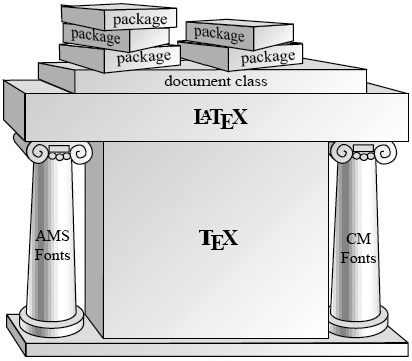
\includegraphics[width=0.45\textwidth]{latexframe}\\\vfill
      
\includegraphics[width=0.35\textwidth]{titlepage}\\%scale=0.05
      贴心\alert{秘书}
    \end{center}
  \end{columns}
  %\end{spacing}
\end{frame}

\begin{frame}{为什么要用\LaTeX?}{Office的那点事}%
  \centering
  
\includegraphics[height=.65\textheight]{msoffice2013.png}\\[.5em]
  \msoffice{} \footnote[frame,1]{及其类似软件(LibreOffice, etc.)}%为了在
                                %beamer中显示脚注,需要使用参数[frame]
  功能异常强大$\cdots$
\end{frame}

\begin{frame}{为什么要用\LaTeX?}{与Word比较}
  \begin{itemize}
  \item 使用难度
  \end{itemize}
  \centering
  \vspace{2ex}
  \begin{tikzpicture}[scale=0.9, every node/.style={scale=0.9}]
    \pgfplotsset{every axis/.append style={line width=1pt}}
    \begin{axis}[%
      axis x line=bottom,
      axis y line=left,
      ymin=0,
      xtick={},
      xticklabels={},
      xlabel near ticks,
      ytick={},
      yticklabels={},
      ylabel near ticks,
      xlabel={文档大小和复杂性\footnote[frame]{\href{http://www.pinteric.com/miktex.html}{Marko
      Pinteric: http://www.pinteric.com/miktex.html}}},
      ylabel={耗时和难度},
      ]
      \begin{scope}[decoration={random steps,segment length=1pt,amplitude=0.1pt},decorate]
        \addplot [msofficecolour, samples=130, domain=0:2] {1+2*x^3}
                  node[near end, sloped, above] {\msoffice}
                  node[anchor=east, pos=.98] {\tiny (我不玩了!再见$\cdots$)};
         \addplot [latexcolour, samples=130, domain=0:2] {2+x}
                  node[near end, sloped, above] {\latex};
      \end{scope}
    \end{axis}
  \end{tikzpicture}
\end{frame}

\begin{frame}{为什么要用\LaTeX?}{与Word比较}
  \begin{itemize}
  \item 学习曲线
  \end{itemize}
  \centering
  \vspace{2ex}
  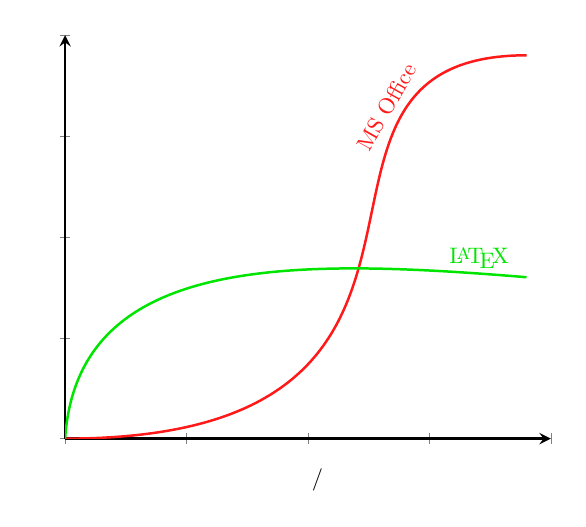
\begin{tikzpicture}[scale=0.9, every node/.style={scale=0.9}]
    \pgfplotsset{every axis/.append style={line width=1pt}}
    \begin{axis}[%
      axis x line=bottom,
      axis y line=left,      
      xtick={},
      xticklabels={},
      xlabel near ticks,
      ytick={},
      yticklabels={},
      ylabel near ticks,
      xlabel={需求复杂度/经验},
      ylabel={学习难度},
      xmin=0,
      xmax=4,
      ymin=0,
      ymax=4,
      ]
      % 用贝塞尔曲线(Bézier curve)绘制学习曲线示意图
      \begin{scope}[decoration={random steps,segment length=1pt,amplitude=0.1pt},decorate]
        \draw[color=msofficecolour] (0,0) .. controls (3.8,0.00) and (1.5,3.8)
        .. (3.8,3.8) node[near end, sloped, above] {\msoffice};
        \draw[latexcolour] (0,0) .. controls (0.1,1.8) and (1.8,1.8)
        .. (3.8,1.6) node[xshift = -0.8cm, sloped, above] {\latex};
      \end{scope}
    \end{axis}
  \end{tikzpicture}
\end{frame}

\begin{frame}{为什么要用\LaTeX?}{Word的那点事}
  \stretchon
  \begin{itemize}
  \item \msoffice 是 \wysiwyg
    \begin{itemize}
    \item ``\textsc{What You See Is What You \emph{Get}}''
    \item 格式和结构有时是含蓄的
    \item 貌似易用,但对排版只能进行有限的控制
    \end{itemize}
    %\myrule
  \item \latex 是 \wysiwym
    \begin{itemize}
    \item ``\textsc{What You See Is What You \emph{Mean}}''
    \item 格式与结构清晰
    \item 貌似繁琐,实则是对版面可以进行详细的控制
    \end{itemize}
  \end{itemize}
  \stretchoff
\end{frame}

\begin{frame}{为什么要用\LaTeX?}{Word的那点事}
  \stretchon
  \begin{itemize}
  \item 玻璃瓶和塑料瓶
    \begin{itemize}
    \item \msoffice 玻璃瓶$\Rightarrow$ \alert{易碎} VS. \latex 塑料瓶$\Rightarrow$ \alert{皮实}
    \end{itemize}
  \item 模板
    \begin{itemize}
    \item \msoffice 往往是\alert{规定}$\Rightarrow$ 沦落为低级趣味的\alert{格式刷}
    \item \latex 强制使用模板$\Rightarrow$ 真正实现了\alert{内容与格式的分离}
    \end{itemize}
  \item 轮子的故事
    \begin{itemize}
    \item \msoffice$\Rightarrow$ \alert{ 发明和制造}轮子  VS. \latex$\Rightarrow$  \alert{ 使用}轮子
    \end{itemize}
  \item 两条腿走路
    \begin{itemize}      
    \item 不会用
      \begin{itemize}
      \item \msoffice $\Rightarrow$ 文档难看,格式丑
      \item \latex $\Rightarrow$ 无法编译,\alert{没有文档}
      \end{itemize}
    \item 会用
      \begin{itemize}
      \item \msoffice $\Rightarrow$ \alert{难看}的文档
      \item \latex $\Rightarrow$ 漂亮的文档
      \end{itemize}
    \item 用的好
      \begin{itemize}
      \item \msoffice $\Rightarrow$ \alert{完美}的文档
      \item \latex $\Rightarrow$ \alert{完美}的文档
      \end{itemize}
    \end{itemize}    
  \end{itemize}
  \stretchoff
\end{frame}

\begin{frame}[fragile]{为什么要用\LaTeX?}{简洁输入优美公式}
  \begin{itemize}
  \item 数学公式\\
    \centering    
    \begin{minipage}{1.0\linewidth}
        \begin{texcode}
                    $$\sum_{p\rm\;prime}f(p) = \int_{t>1}f(t)d\pi(t).$$
                \end{texcode}
    \end{minipage}\\
    \begin{minipage}[h]{0.95\linewidth}
      $$\sum_{p\rm\;prime}f(p) = \int_{t>1}f(t)d\pi(t).$$
    \end{minipage}\\
    \begin{minipage}[h]{1.\linewidth}
      \begin{texcode}
                $$2\uparrow\uparrow k
                \mathrel{\mathop=^{\rm def}}
                2^{2^{\cdot^{\cdot^{\cdot^2}}}}
                \vbox{\hbox{$\Big\}\scriptstyle k$}\kern0pt}.$$
            \end{texcode}
    \end{minipage}\\%[1.3em]
    \begin{minipage}[h]{0.95\linewidth}
      $$2\uparrow\uparrow k
      \mathrel{\mathop=^{\rm def}} 2^{2^{\cdot^{\cdot^{\cdot^2}}}}
      \vbox{\hbox{$\Big\}\scriptstyle k$}\kern0pt}.$$
    \end{minipage}
  \end{itemize}
\end{frame}

\begin{frame}[t,fragile]{为什么要用\LaTeX?}{优雅地绘图}
  \begin{tabular}{cc}
      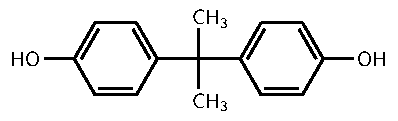
\includegraphics[width=.45\textwidth]{tikzexample/chem.pdf}
    &
      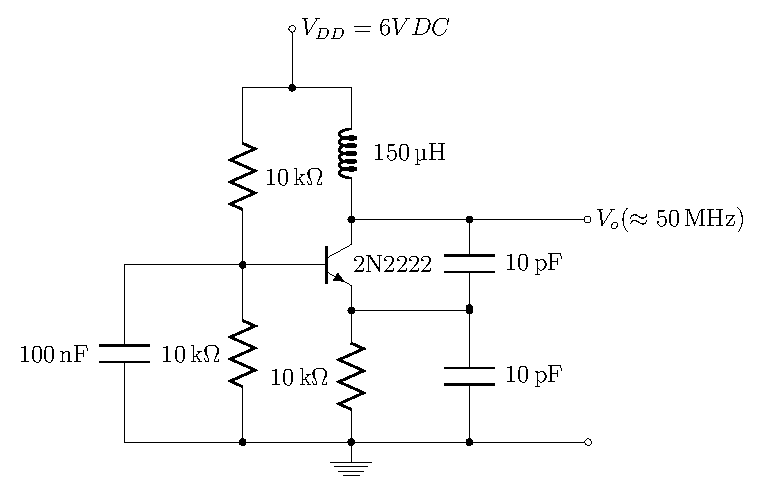
\includegraphics[width=.45\textwidth]{tikzexample/circuitikz.pdf}\\
    
      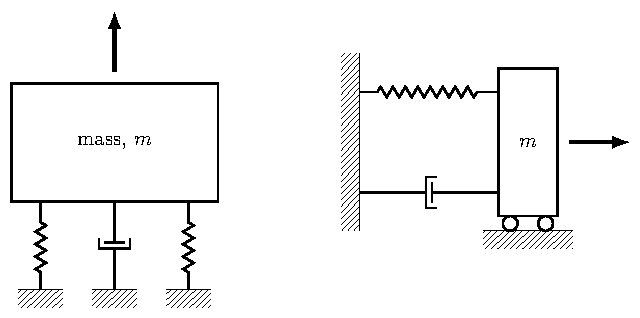
\includegraphics[width=.45\textwidth]{tikzexample/mechanicalsys.pdf}
    &
      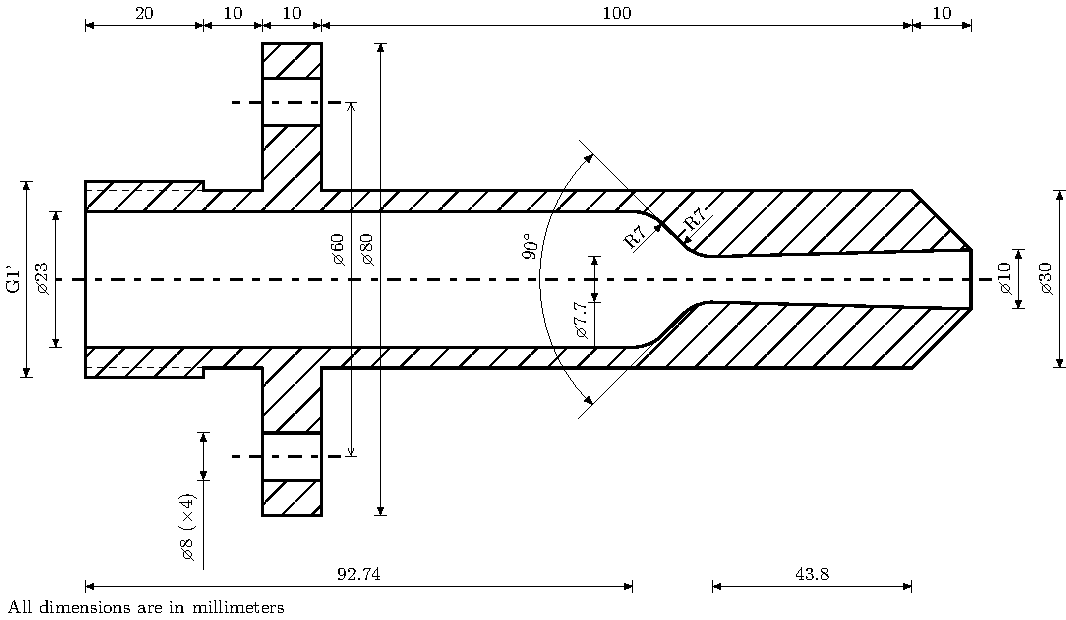
\includegraphics[width=.45\textwidth]{tikzexample/tecdraw.pdf}
  \end{tabular}
\end{frame}

\subsection[是什么?]{什么是\LaTeX ?}\label{sec01-02}
\begin{frame}[t]{什么是\LaTeX?}{排版准备系统}
  \stretchon
  \begin{itemize}
  \item \LaTeX{}是一个功能强大的排版准备系统
  \item \LaTeX{}是标记型语言系统
  %\item \wysiwym
  \item 基于\TeX
    \begin{itemize}
    \item \TeX{}系统提供了300多条基本的排版命令
    \item 允许用户自定义新命令
    \end{itemize}
  \item 大量适合领域排版的宏包(CTAN\link{www.ctan.org},
    \alert{5881}个,\today )
  \end{itemize}
  \stretchoff
\end{frame}

\begin{frame}[t]{什么是\LaTeX?}{工作流程}
  %\stretchon
  \begin{itemize}
  \item \wysiwym\\[4ex]
    %\begingroup
    %\centering
    \begin{center}
      \begin{tikzpicture}[shorten >=1pt,node distance=3cm,auto]
        \draw[%
        -open triangle 60,%
        very thick, ] (0,0) node[anchor=east] (tex)
        {
\includegraphics[height=.2\textheight]{tex_file.png}} --
        (3,0) node[anchor=west] (pdf)
        {
\includegraphics[height=.2\textheight]{pdf_file.png}};
      \end{tikzpicture}
    %\endgroup
    \end{center}
    \vspace{4ex}
  \item \wysiwyg\\[4ex]
    \begin{center}
      
\includegraphics[height=.2\textheight]{word_file.jpg}
    \end{center}
  \end{itemize}
  %\stretchoff
\end{frame}

\begin{frame}[t, fragile]{什么是\LaTeX?}{工作流程}
  \begin{itemize}
  \item 排版流程
  \end{itemize}
  \centering
  \tikzset{ box/.style = {rectangle, draw=black, fill=lightgray} }
  \begin{tikzpicture}
    \node[box] (tex) at(0,0) {.tex};
    \node[box] (pdf) at(8,0) {.pdf};
    \node[box] (dvi) at(0,-4) {.dvi};
    \node[box] (ps) at(8,-4) {.ps};
    \draw[->,very thick, red] (tex) -- node[above]{\alert{\XeLaTeX}} (pdf);
    \draw[->,very thick, red] (tex) -- node[below]{pdf\LaTeX} (pdf);
    \draw[->] (tex) -- node[right]{\LaTeX} (dvi);
    \draw[->] (dvi) -- node[above]{dvips} (ps);
    \draw[->] (ps) -- node[right]{ps2pdf} (pdf);
    \draw[->] (dvi) -- node[above,sloped]{dvipdfmx} (pdf);
  \end{tikzpicture}
  \begin{center}
    \begin{minipage}{0.6\linewidth}
      \footnotesize
      \begin{block}{编译方案}
        \centering
        一般用{pdf\LaTeX}或者{\XeLaTeX}程序直接生
        成\verb|pdf|文件。\\
        如果是\alert{中文}tex文档,\alert{优先}使用\alert{{\XeLaTeX}}程序编译。
      \end{block}
    \end{minipage}
  \end{center}  
\end{frame}

\begin{frame}[t]{什么是\LaTeX?}{特点}
  \stretchon
  \begin{itemize}
  \item 自动编号:一切需要皆有可能
  \item 自动生成目录、索引
  \item 交叉引用:公式、定理、文献、插图、页码等等
  \item PDF输出
  \item 参考文献库
  \item 扩展宏包
  \item $\cdots\cdots$
  \end{itemize}
  \stretchoff
\end{frame}

\begin{frame}[t, fragile]{什么是\LaTeX?}{自动化处理---简单文档}
  \begin{itemize}
  \item 单次编译[xelatex jobname]
  \end{itemize}
  \vfill
  \begin{center}
    \begin{tikzpicture}[font=\scriptsize, ,scale=\scaleratio, every node/.style={scale=\scaleratio}]
      \node[proc, fill=blue!30](src){.tex源文档};
      \node[proc, join, fill=yellow!30](tex){{\LaTeX}引擎};
      \node[proc, join, text width = 5.1em](notocpdf){PDF排版结果};
      \node[proc, below=1.5 of tex, text width = 6.5em, fill=green!30, dashed](aux){.aux(辅助文件)};

      \path (src.east) to node[cirnum, above, fill=black] {\tiny 1} (tex);
      \path (tex.east) to node[cirnum, above, fill=black] {\tiny 1} (notocpdf);
      \draw [free, dashed, green!50] (tex.south) -- node[cirnum, right, fill=lightgray] {\tiny 1}(aux.north);
    \end{tikzpicture}
  \end{center}
  \vfill
\end{frame}

\begin{frame}[t, fragile]{什么是\LaTeX?}{自动化处理---图表引用}
  \begin{itemize}
  \item 两次编译[xelatex jobname/xelatex jobname]
  \end{itemize}
  \vfill
  \begin{center}
    \begin{tikzpicture}[font=\scriptsize, scale=\scaleratio, every node/.style={scale=\scaleratio}]
      \node[proc, fill=blue!30](src){.tex源文档};
      \node[proc, join, fill=yellow!30](tex){{\LaTeX}引擎};
      \node[proc, join, text width = 5.1em](notocpdf){无交叉引用PDF\\(带``??''PDF)};
      \node[proc, below=1.5 of tex, text width = 6.5em, fill=green!30, dashed](aux){.aux(辅助文件)};
      \node[proc, below=3.0 of tex, fill=yellow!30](btex){{\LaTeX}引擎};
      \node[proc, join, text width = 6.5em, fill=red!40](pdf){.pdf(排版结果)};

      \path (src.east) to node[cirnum,fill=black] {\tiny 1} (tex);
      \path (tex.east) to node[cirnum,fill=black] {\tiny 1} (notocpdf);
      \draw [free, dashed, green!50] (tex.south) -- node[cirnum, right, fill=lightgray] {\tiny 1}(aux.north);
      \draw [cong, dashed, red!50] (aux.south) -- node[cirnum, right, fill=lightgray] {\tiny 2}(btex.north);
  
      \draw [norm] (src.south) to [in=180, out=-90]node[cirnum, shift={(0.15em, 0.15em)},fill=black] {\tiny 2}(btex);
      \path (btex.east) to node[cirnum,fill=black] {\tiny 2} (pdf.west);
    \end{tikzpicture}
  \end{center}
  \vfill
\end{frame}

\begin{frame}[t, fragile]{什么是\LaTeX?}{自动化处理---目录}
  \begin{itemize}
  \item 两次编译[xelatex jobname/xelatex jobname]
  \end{itemize}
  \vfill
  \begin{center}
    \begin{tikzpicture}[font=\scriptsize, scale=\scaleratio, every node/.style={scale=\scaleratio}]
      \node[proc, fill=blue!30](src){.tex源文档};
      \node[proc, join, fill=yellow!30](tex){{\LaTeX}引擎};
      \node[proc, join](notocpdf){无目录PDF};
      \node[proc, below=1.5 of tex, text width = 4.6em, fill=green!30, shift={(-1.0,0.0)}, dashed](aux){.aux\\(辅助文件)};
      \node[proc, right=3.0 of aux, text width = 4.5em, fill=green!30, dashed](toc){.toc/.lot/.lof\\(目录文件)};
      \node[proc, below=3.0 of tex, fill=yellow!30](btex){{\LaTeX}引擎};
      \node[proc, join, text width = 6.5em, fill=red!40](pdf){.pdf(排版结果)};

      \path (src.east) to node[cirnum,fill=black] {\tiny 1} (tex);
      \path (tex.east) to node[cirnum,fill=black] {\tiny 1} (notocpdf);
      \draw [free, dashed, green!50] (tex.south) -- node[cirnum, fill=lightgray] {\tiny 1}(aux.north);
      \draw [free, dashed, green!50] (tex.south) -- node[cirnum, fill=lightgray] {\tiny 1}(toc.north);
      \draw [cong, dashed, red!50] (aux.south) -- node[cirnum, shift={(-0.4em, -0.5em)}, fill=lightgray] {\tiny 2}(btex.north);
      \draw [cong, dashed, red!50] (toc.south) -- node[cirnum, shift={(0.4em, -0.5em)}, fill=lightgray] {\tiny 2}(btex.north);
  
      \draw [norm] (src.south) to [in=180, out=-90]node[cirnum,fill=black, shift={(0.15em, 0.15em)}] {\tiny 2}(btex);
      \path (btex.east) to node[cirnum,fill=black] {\tiny 2} (pdf.west);
    \end{tikzpicture}
  \end{center}
  \vfill
\end{frame}

\begin{frame}[t, fragile]{什么是\LaTeX?}{自动化处理---Bibtex处理参考文献}
  \begin{itemize}
  \item 四次编译[\small xelatex jobname/bibtex jobname/xelatex jobname/xelatex jobname]
  \end{itemize}
  \vfill
  \begin{center}
    \def\scaleratio{1.0}
    \begin{tikzpicture}[font=\scriptsize, scale=\scaleratio, every node/.style={scale=\scaleratio}]
      \node[proc, fill=yellow!30](tex){{\LaTeX}引擎};
      \node[proc, join](nobibpdf){无文献PDF};
      \node[proc, below=1.0 of nobibpdf, text width = 5.5em, fill = violet!40, shift = {(-1.0, 0.0)}](bib){.bib文献数据库};
      \node[proc, right=3.0 of bib, text width = 4.6em, fill = violet!40](bst){.bst文献样式};
      \node[proc, below=2.0 of tex, text width = 5em, fill=green!30, dashed](aux){.aux(辅助文件)};
      \node[proc, right=3.3 of aux, text width = 4.5em, fill=yellow!30](bibtex){bibtex工具};
      \node[proc, right=3.0 of bibtex, text width = 4.5em, fill=green!30, dashed](bbl){.bbl文献列表};
      \node[proc, below=1.2 of aux, fill=yellow!30](btex){{\LaTeX}引擎};  
      \node[proc, join, text width = 4.5em](norefpdf){无引用PDF};
      \node[proc, left = 3.2 of btex, fill=blue!30](src){.tex源文档};
      \node[proc, below=1.2 of btex, text width = 6.5em, fill=green!30, dashed](baux){.aux(辅助文件)};
      \node[proc, below=1.2 of baux, fill=yellow!30](bbtex){{\LaTeX}引擎};
      \node[proc, join, text width = 4.5em, fill=red!60](pdf){最终PDF};

      \path (tex.east) to node[cirnum, fill=black] {\tiny 1} (nobibpdf);
      \path (tex.east) to node[cirnum, fill=black] {\tiny 1} (nobibpdf);
      \path (btex.east) to node[cirnum, fill=black] {\tiny 3} (norefpdf);
      \path (bbtex.east) to node[cirnum, fill=black] {\tiny 4} (pdf);
  
      \draw[norm] (src) -- node[cirnum, below, fill=black]{\tiny 3} (btex);
      \draw[norm] (src) edge [bend left] node[cirnum, right, fill=black]{\tiny 1} (tex);
      \draw[norm] (src) edge [bend right] node[cirnum, right, fill=black]{\tiny 4} (bbtex);

      \draw[free, dashed, green!80] (tex.south) -- node[cirnum, fill=lightgray] {\tiny 1}(aux.north);
      \draw[free, dashed, red!40] (aux) -- node[cirnum, fill=lightgray] {\tiny 2}(bibtex);
      \draw[free, dashed, green!80] (bibtex) -- node[cirnum, fill=lightgray] {\tiny 2}(bbl); 
      \draw[norm] (bib.south) -- node[cirnum, below, fill=black]{\tiny 2} (bibtex.north);
      \draw[norm] (bst.south) -- node[cirnum, below, fill=black]{\tiny 2} (bibtex.north);
  
      \draw[free, dashed, red!40] (aux) -- node[cirnum, fill=lightgray] {\tiny 3}(btex);
      \draw[free, dashed, red!40] (bbl.south) -- node[cirnum, fill=lightgray] {\tiny 3}(btex.north);

      \draw[free, dashed, green!80] (btex.south) -- node[cirnum, fill=lightgray] {\tiny 3}(baux.north);
      \draw[free, dashed, red!40] (baux.south) -- node[cirnum, fill=lightgray] {\tiny 4}(bbtex.north); 
      \draw[free, dashed, red!40] (bbl.south) to [out=-90, in = 45] node[cirnum, fill=lightgray] {\tiny 4}(bbtex.north east); 
    \end{tikzpicture}
  \end{center}
  \vfill
\end{frame}

\begin{frame}[t, fragile]{什么是\LaTeX?}{自动化处理---Biber处理参考文献}
  \begin{itemize}
  \item 四次编译[\small xelatex jobname/biber jobname/xelatex jobname/xelatex jobname]
  \end{itemize}
  \vfill
  \begin{center}
    \def\scaleratio{1.0}
    \begin{tikzpicture}[font=\scriptsize, scale=\scaleratio, every node/.style={scale=\scaleratio}]
      \node[proc, fill=yellow!30](tex){{\LaTeX}引擎};
      \node[proc, join](nobibpdf){无文献PDF};
      \node[proc, below = 1.0 of tex, text width = 4.5em, fill=yellow!30, dashed, shift={(3.0, 0.0)}](sty){biblatex宏包};
      \node[proc, text width = 10.0em, fill=violet!40](bbxcbx){.bbx著录样式/.cbx引用样式};
      \node[proc, below=2.5 of tex, text width = 5.0em, fill=green!30, dashed](aux){.aux(辅助文件)};
      \node[proc, right=2.5 of aux, text width = 5.0em, fill=green!30, dashed](bcf){.bcf(引用文件)};
      \node[proc, right=2.8 of bcf, text width = 4.5em, fill=yellow!30](biber){biber工具};
      \node[proc, right=2.8 of biber, text width = 5.5em, fill = violet!40](bib){.bib文献数据库};
      \node[proc, above=0.75 of biber, text width = 4.5em, fill=green!30, dashed, shift = {(-0.6, 0.0)}](bbl){.bbl文献列表};
      \node[proc, below=1.2 of aux, fill=yellow!30](btex){{\LaTeX}引擎};  
      \node[proc, join, right=4.5 of btex, text width = 4.5em, fill=red!60](norefpdf){带文献PDF};
      \node[proc, left = 3.2 of btex, fill=blue!30](src){.tex源文档};  
      \node[proc, below=1.2 of btex, fill=yellow!30](bbtex){{\LaTeX}引擎};
      \node[proc, join, text width = 8.0em, fill=red!80](pdf){带文献反向超链接PDF};

      \path (tex.east) to node[cirnum, fill=black] {\tiny 1} (nobibpdf);
      \path (btex.east) to node[cirnum, fill=black] {\tiny 3} (norefpdf);
      \path (bbtex.east) to node[cirnum, fill=black] {\tiny 4} (pdf);
  
      \draw[norm] (src) -- node[cirnum, below, fill=black]{\tiny 3} (btex);
      \draw[norm] (src) edge [bend left] node[cirnum, right, fill=black]{\tiny 1} (tex);
      \draw[norm] (src) edge [bend right] node[cirnum, right, fill=black]{\tiny 4} (bbtex);

      \draw[free, violet!80] (bbxcbx.west) -- node[cirnum, xshift=-0.6em, fill=black]{\tiny 1}(sty.east);
      \draw[free, violet!80] (bbxcbx.west) -- node[cirnum, fill=black]{\tiny 3}(sty.east);
      \draw[free, violet!80] (bbxcbx.west) -- node[cirnum, xshift=0.6em, fill=black]{\tiny 4}(sty.east);

      \draw[norm, dashed] (sty.north west) -- node[cirnum, fill=black]{\tiny 1} (tex.south east);
  
      \draw[free, dashed, green!80] (tex.south) -- node[cirnum, fill=lightgray] {\tiny 1}(bcf.north);
      \draw[free, dashed, green!80] (tex.south) -- node[cirnum, fill=lightgray] {\tiny 1}(aux.north);
      \draw[free, dashed, red!40] (bcf.east) -- node[cirnum, fill=lightgray] {\tiny 2}(biber.west);
      \draw[free, dashed, green!80] (biber) -- node[cirnum, fill=lightgray] {\tiny 2}(bbl); 
      \draw[norm] (bib) -- node[cirnum, fill=black]{\tiny 2} (biber);
  
      \draw[free, dashed, red!40] (bbl.north) -- node[cirnum, fill=lightgray] {\tiny 3}(sty.south);
      \draw[norm, dashed] (sty.south)  to [out=-90, in = 45] node[cirnum, near end, fill=black]{\tiny 3} (btex.north east);
      \draw[norm, dashed] (sty.south) to [out=-90, in = 45] node[cirnum, near end, fill=black]{\tiny 4} (bbtex.north east);

      \draw[free, dashed, red!40] (aux.south) -- node[cirnum, fill=lightgray] {\tiny 4}(btex.north);
      \draw[norm, dashed, red!40] (aux.south east) to [out=-45, in = 45] node[cirnum, near end, fill=black]{\tiny 4} (bbtex.north);
    \end{tikzpicture}
  \end{center}
  \vfill
\end{frame}

\begin{frame}[fragile]{什么是\LaTeX?}{特点}%, label=testframe
  %\stretchon
  \begin{itemize}
  \item 内容与样式分离\footnote[frame]{\href{https://liam.page/2019/03/18/separation-of-content-and-presentation/}{https://liam.page/2019/03/18/separation-of-content-and-presentation/}}
  \end{itemize}  
  \begin{center}
  \begin{minipage}[c]{0.9\linewidth}
    
\includegraphics[width=1.0\textwidth]{theorem}    
  \end{minipage}
  \end{center}
  \vspace{-1ex}
  \begin{spacing}{1.05}
  \begin{columns}[T]
    \column{0.3\linewidth}
    \begin{itemize}
    \item 不分离实现      
      \begin{enumerate}
        \scriptsize
      \item 加粗
      \item \enquote{定理}
      \item \enquote{空格}
      \item 数字 \enquote{1}
      \item 左括号\enquote{(}
      \item \enquote{勾股定理}
      \item 右括号\enquote{)}
      \item 句点\enquote{.}
      \item \enquote{空格}
      \item 结束加粗
      \item 倾斜体
      \item \enquote{定理文本...}
      \item 结束倾斜
      \end{enumerate}
    \end{itemize}
    \column{0.65\linewidth}
    \begin{itemize}
    \item 分离实现
      \begin{enumerate}
        \scriptsize
      \item 这是一个定理
      \item 它的编号是1
      \item 它的名称是\enquote{勾股定理}
      \item 它的内容是\enquote{定理文本...}
      \item 分别\alert{放在恰当的标记中}
      \end{enumerate}
      %\vspace{-1.5ex}
      \begin{minipage}[h]{0.8\linewidth}
        %\begin{exampleblock}{示例}
          %\vspace{-2ex}
          \begin{texcode*}{fontsize=\tiny}
           % 导言区
           \usepackage{amsmath}
           \newtheorem{theorem}{定理}
           ...
           \begin{theorem}[勾股定理]
             设直⻆三⻆形的三条边⻓分别是$a$, $b$和 $c$ , 
             其中 $c$ 是斜边边⻓,则有 $a^2 + b^2 = c^2$ 成立.
           \end{theorem}
         \end{texcode*}
        %\end{exampleblock}
       \end{minipage}        
    \end{itemize}
  \end{columns}
  \end{spacing}
  % %\stretchoff
\end{frame}

\begin{frame}[t]{什么是\LaTeX?}{优点}
  \stretchon
  \begin{itemize}
  \item {\color{blue}{高质量的输出:}}\LaTeX{}以排版质量为首要目标
  \item {\color{blue}{超常的稳定性:}}\LaTeX{}系统极少崩溃
  \item {\color{blue}{\LaTeX{}是宏命令编程语言:}}用命令完成排版
    (可自定义或重定义)
  \item {\color{blue}{\LaTeX{}是纯文本文件:}}占用空间很小
  \item {\color{blue}{良好的通用性和低廉的价格:}}免费
  \item {\color{blue}{超强的技术支持:}}丰富的网络资源
  \end{itemize}
  \stretchoff
\end{frame}

\begin{frame}[t]{什么是\LaTeX?}{协作}
  \vspace{-3ex}
  \begin{columns}[t]
    \column{0.35\textwidth}
  \begin{spacing}{0.7}
    \begin{itemize}
    \item \alert{多人}
      \begin{itemize}
      \item 明文编辑
        \begin{itemize}
        \item 方便自由
        \end{itemize}
      \item 版本管理
        \begin{itemize}
        \item 安全可靠
        \item 回滚便捷
        \end{itemize}
      \item 模板丰富
        \begin{itemize}
        \item 实习报告/论文
        \item 科研论文
        \item 学位论文
        \end{itemize}
      \end{itemize}
    \item \alert{多文件}
      \begin{itemize}
      \item 分章节协作
      \item 分专题协作
      \item 分模块协作
      \end{itemize}
    \item \alert{软件}
      \begin{itemize}
      \item 图文分离
        \begin{itemize}
        \item 独立编辑
        \end{itemize}
      \item 表文分离
        \begin{itemize}
        \item 数据文件
        \end{itemize}
      \end{itemize}
    \end{itemize}
  \end{spacing}
  \column{0.65\textwidth}
  \vspace{-2.0ex}
  \begin{center}
    % \includegraphics[height=0.8\textheight]{coworks}
    \scalebox{0.5}{
      %  \begin{center}
    % \includegraphics[height=0.8\textheight]{coworks}
%    \scalebox{0.5}{
      \begin{forest}
        pic dir tree,
        pic root,
        for tree={% folder icons by default; override using file for file icons
          directory,
        },
        [jobname【工作根目录】%, 
          [bib【参考文献数据库目录,根据需要,可以有多个数据库】%
            [sample.bib【样例数据库,根据需要,可以有多个数据库】, file%
            ]   
          ]
          [codes【报告中需要的代码源文件,可以有多个,根据需要增减】        
            [ex04-01.cpp, file
            ]
            [$\vdots$, file
            ]
          ]
          [figs【插图目录,可根据需要增减】
            [plot
            ]
            [xxxx.png, file
            ]
            [xxxx.pdf, file
            ]
          ]
          [settings【自定义命令、环境等文件、引入宏包文件,可根据需要进行调整】        
            [format.tex【自定义命令、环境、参数设置等】, file
            ]
            [math-commands.tex【自定义数学符号命令】, file
            ]
            [packages.tex【需要引入的宏包】, file
            ]
            [terms.tex【自定义术语命令】, file
            ]
          ]
          [boxie.sty【盒子宏包,如果需要则置于根目录,并在settings/package.tex中引用该宏包】, file
          ]
          [fvextra.sty【子宏包需要的宏包,如果使用了boxie宏包,则必须置于根目录】, file
          ]
          [lstlinebgrd.sty【子宏包需要的宏包,如果使用了boxie宏包,则必须置于根目录】, file
          ]
          [main.tex【主控文件,\emph{必须存在},且置于根目录】, file
          ]
          [Makefile【ake命令需要的脚本文件,如能执行make,可以在根目录执行make命令进行编译】, file
          ]
          [nwafuprojrep.cls【文档类文件,即模板文件,必须存在,且置于根目录】, file
          ]
          [pgf-umlcd.sty【UML图绘制宏包,如果需要则置于根目录,并在settings/package.tex中引用该宏包】, file
          ]
          [tikz-flowchart.sty【流程图绘制宏包,如果需要则置于根目录,并在settings/package.tex中引用该宏包】, file
          ]
          [tikz-imglabels.sty【图像标注/标记宏包,如果需要则置于根目录,并在settings/package.tex中引用该宏包】, file
          ]
          [.latexmkrc【latexmk命令需要的脚本文件,如能执行latexmk,可以在根目录执行latexmk命令进行编译】, file
          ]
        ]
      \end{forest}
%    }
%  \end{center}

    }
  \end{center}
\end{columns}
\end{frame}

\begin{frame}[t]{什么是\LaTeX?}{缺点}
  \stretchon
  \begin{itemize}
  \item 命令繁多
    \begin{itemize}
    \item 常备一本参考资料
    \item 要\alert{多用}
    \end{itemize}
  \item 错误难找:积累经验
  \item 写宏包有难度:普通用户不需要自己写宏包
  \item 使用不直观:目前已有一些所见即所得的扩展
  \end{itemize}
  \stretchoff
\end{frame}

\begin{frame}[t]{什么是\LaTeX?}{PDF文件的批阅批注}
  %\vspace{-3ex}
  % \stretchon
  \begin{columns}[c]
    % \column{0.05\textwidth}
    \column{0.5\textwidth}
    \begin{spacing}{0.9}
    \begin{itemize}%[noitemsep]
    \item \alert{纸质}批注\footnote[frame]{保留\alert{真迹},以作纪念!}
      \begin{itemize}
      \item 打印
      \end{itemize}
    \item
      \alert{平板}批注\footnotemark[\value{footnote}]%\footnotemark[\ref{note
      \begin{itemize}
      %\item GoodNotes
      \item Notability
      \item $\cdots$
      \end{itemize}
    \item \alert{软件}批注
      \begin{itemize}
      \item Adobe Acrobat Pro
      %\item Foxit Reader(福昕)
      %\item Okular
      \item $\cdots$
      \end{itemize}
    \item \alert{源码}批注\footnote[frame]{导师\qtmark{智慧过人、气
          宇不凡、天资聪颖、骨骼精奇},学习\LaTeX 那是\alert{分分钟
          钟}的事!}
      \begin{itemize}
      \item Git版本管理,diff查看
        \begin{itemize}
        \item {GitHub}\link{https://github.com/}
        \item {码云}\link{https://gitee.com/}
        \end{itemize}
      \item 批注宏包
        \begin{itemize}
        \item changes
        %\item todonotes
        \item $\cdots$
        \end{itemize}
      \end{itemize}
    \end{itemize}
    \end{spacing}
  \column{0.45\textwidth}
  \begin{center}
    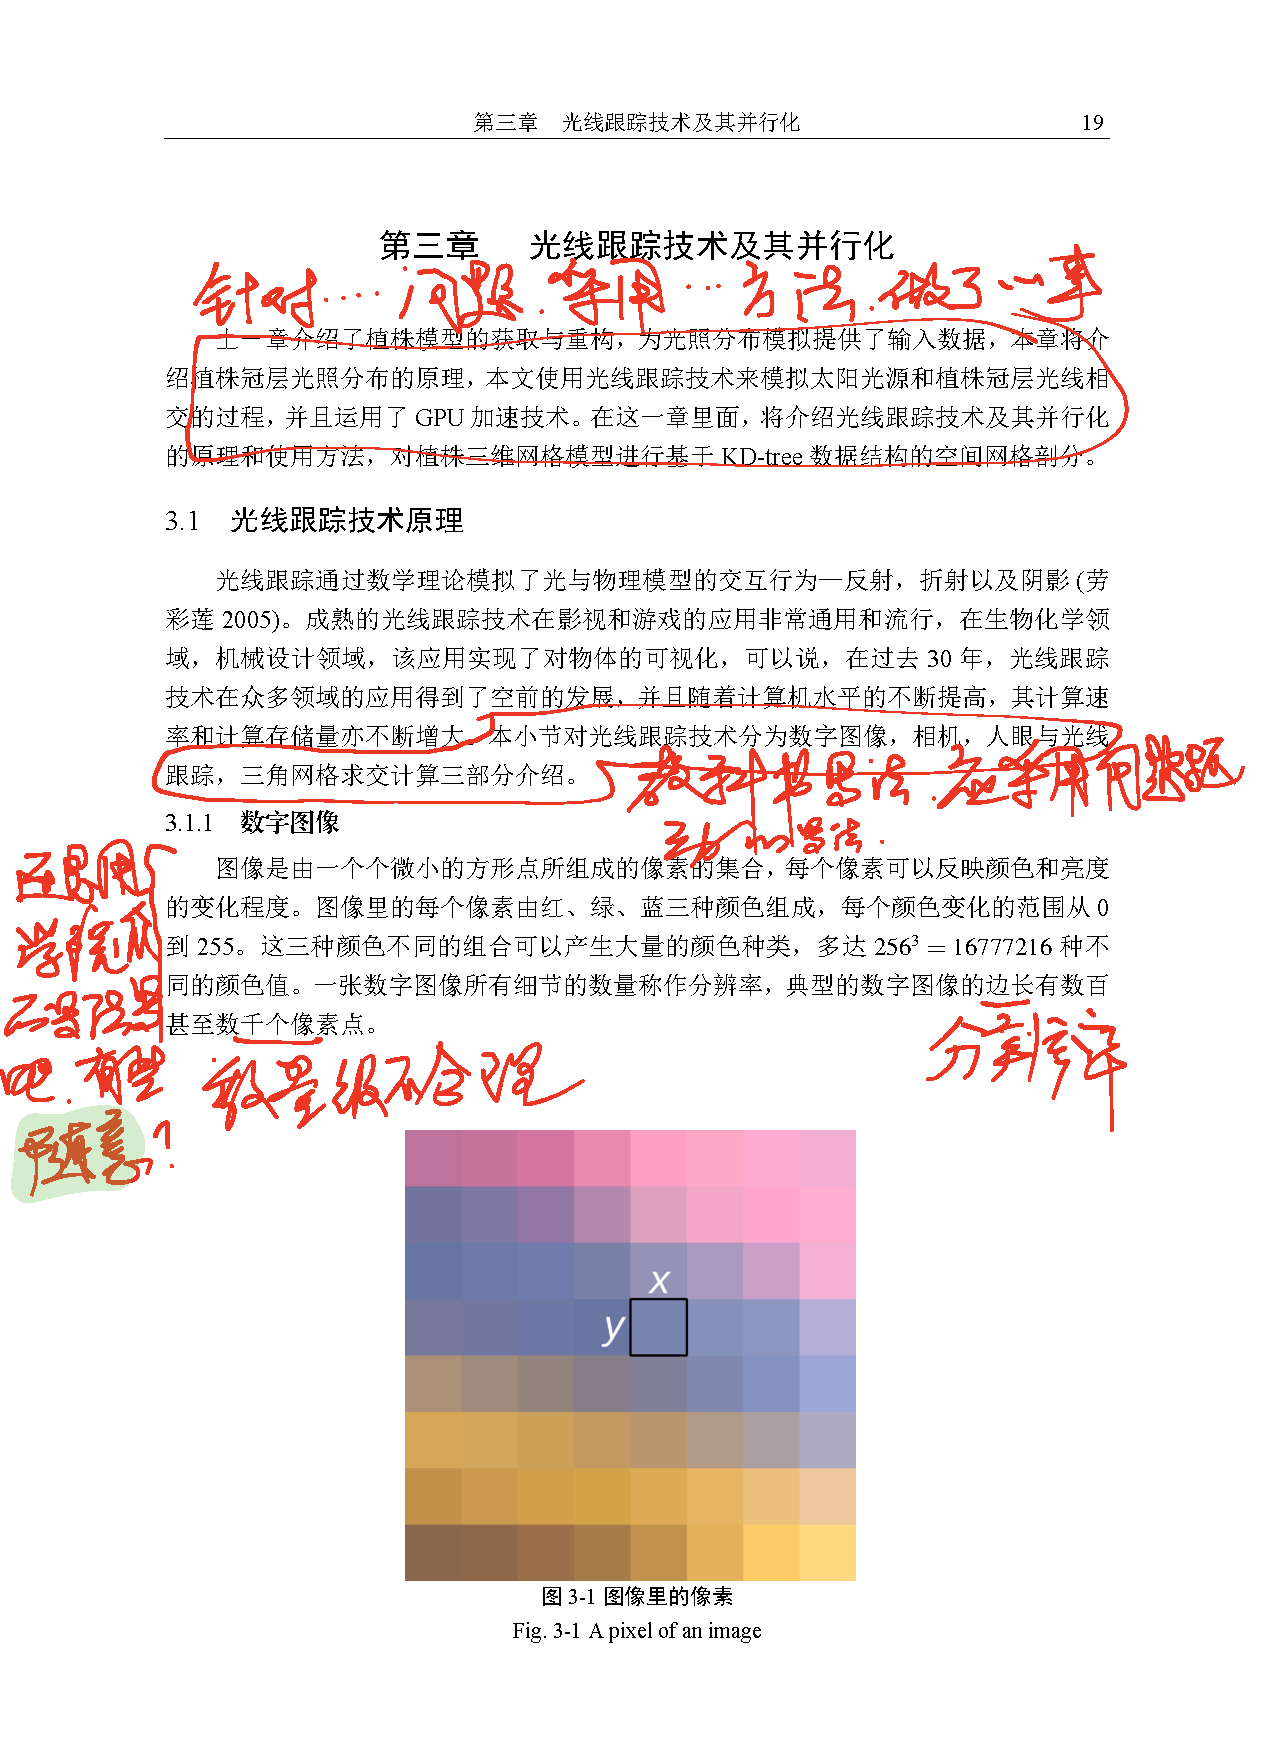
\includegraphics[width=0.4\textwidth]{pdftakenotes}\\
    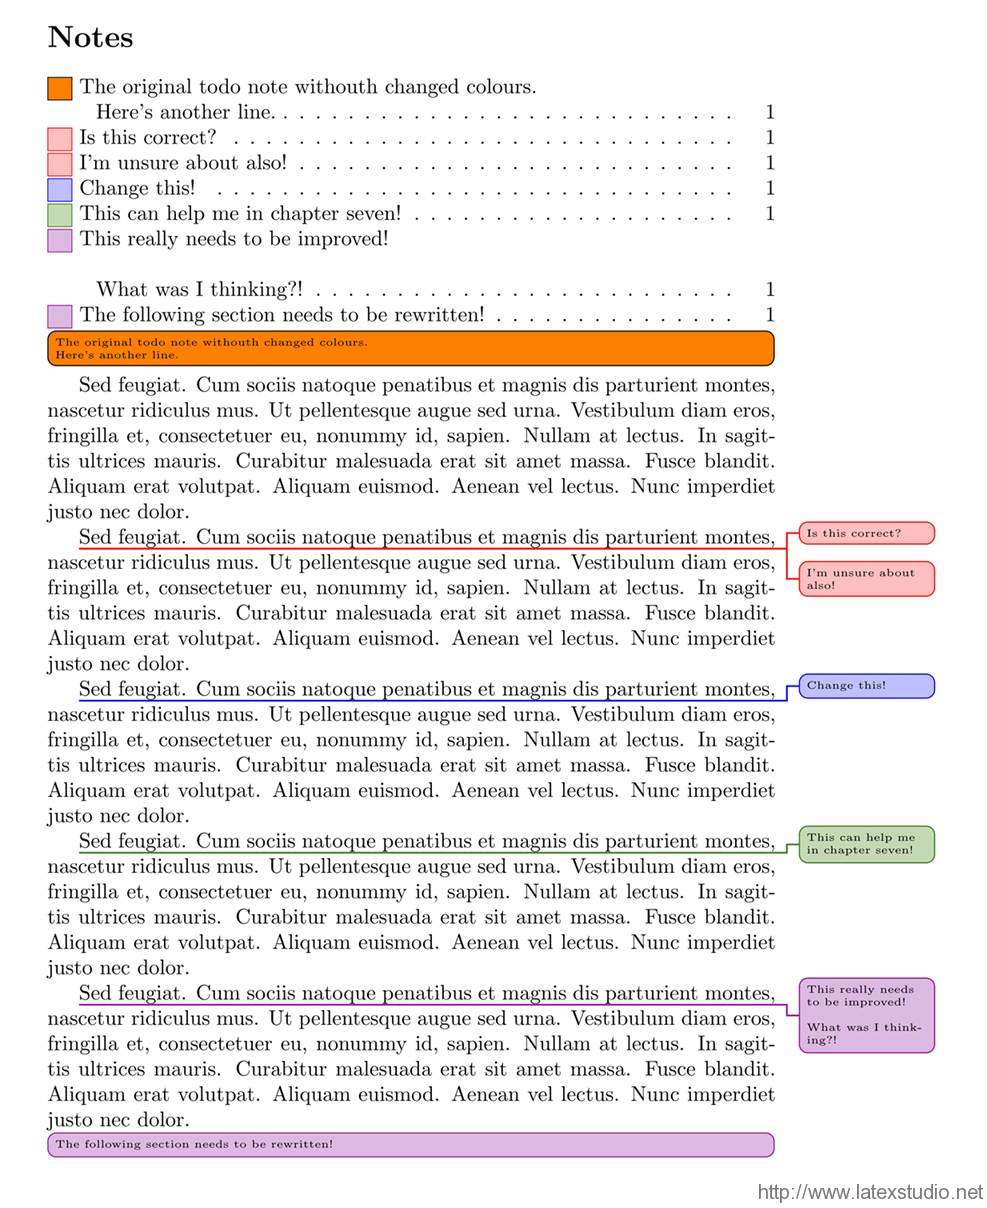
\includegraphics[width=0.4\textwidth]{todonotes}
  \end{center}
\end{columns}
% \stretchoff
\end{frame}

\begin{frame}{什么是\LaTeX?}{基本原则}
  \stretchon
  \begin{itemize}
  \item 排版 vs 文字处理
    \begin{itemize}
    \item 《别把 \LaTeX{} 当 Word 用》
    \end{itemize}
  \item 遵循\alert{学校规范}(业界规范)
    \begin{itemize}
    \item 研究生院/教务处
    \item 教学办
    \item 导师
    \end{itemize}
  \item 追求良好的阅读体验
  \item 内容与格式分离
  \item \alert{内容永远比格式重要!}
  \end{itemize}
  \stretchoff
\end{frame}

\begin{frame}[fragile]{什么是\LaTeX?}{谋篇布局}
  \stretchon
  \begin{itemize}
  \item 文档部件\footnote[frame,1]{本页面摘自曾祥东的\enquote{现代\LaTeX 入门讲座}
      讲义\link{https://github.com/stone-zeng/latex-talk}。}
    \begin{itemize}
    \item 标题:\texinline{\title}、\texinline{\author}、\texinline{\date} $\to$ \texinline{\maketitle}
    \item 摘要:\texinline{abstract} 环境
    \item 目录:\texinline{\tableofcontents}
    \item 章节:\texinline{\chapter}、\texinline{\section}、\texinline{\subsection} 等
    \item 文献:\texinline{\bibliography}
    \end{itemize}
  \item 文档划分
    \begin{itemize}
    \item 凤头猪肚豹尾:\texinline{\frontmatter}、\texinline{\mainmatter}、\texinline{\backmatter}
    \item 分文件编译:\texinline{\include}、\texinline{\input}
    \end{itemize}
  \end{itemize}
  \stretchoff
\end{frame}

\begin{frame}[t]{什么是\latex?}{\latex 的版本}
  \stretchon
  \begin{itemize}
  \item 发行版:
    \begin{itemize}    
    \item Windows:CTex,MikTex,fpTeX
    %\item Unix/Linux:teTeX
    \item Mac OS:MacTeX        
    \item 跨平台:\alert{TeXlive}\link{https://www.tug.org/texlive/},由国际{\TeX}用户组织开发
    \end{itemize}
  \item 编辑器:
    \begin{itemize}
    \item WinEdt,windows平台,收费
    \item \alert{TexStudio},跨平台,免费
    % \item Lyx,跨平台,免费
    \item TexMacs,Mac平台,免费
    % \item Gummi,Linux平台,免费
    % \item Kile,Lunix平台,免费
    \item $\cdots\cdots$
    \end{itemize}
  \item 在线系统
    \begin{itemize}
    \item
      {ShareLaTeX}: \link{https://cn.sharelatex.com/}
    \item
      {Overleaf}: \link{https://www.overleaf.com/}
    \item
      {Overleaf V2}: \link{https://v2.overleaf.com/}
    \end{itemize}
  \item \alert{不要安装\CTeX{} 套装!} \link{http://www.ctex.org/HomePage}
    \begin{itemize}
      \item \alert{存在严重 bug,并且完全过时}
    \end{itemize}
  \end{itemize}
  \stretchoff
\end{frame}

\begin{frame}[t]{什么是\latex?}{处理中文}
  \stretchon
  \begin{itemize}
  \item \XeTeX 和\XeLaTeX
    \begin{itemize}
    \item 底层支持Unicode
    \item 字体配置方式灵活
    \item \alert{目前最优的中文处理方式!}
    %\item \url{http://scripts.sil.org/xetex}
    \end{itemize}
  \item CCT外挂(\alert{已废弃})
    \begin{itemize}
    \item 中科院张林波开发
    \item 适合中国国情
    \end{itemize}  
  \item CJK外挂(\alert{已废弃})
    \begin{itemize}
    \item 德国人 Werner Lemberg 开发
    \item 中文(\alert{C}hinese)、日文(\alert{J}apanese)、韩文(\alert{K}orean)
    \item 缺乏可用的字体
    \item 默认的格式不符合中文排版要求
    \item 不能满足中文的其他要求
    \end{itemize}  
    %\item \url{ftp://ftp.cc.ac.cn/pub/cct/}      
  \end{itemize}
  \stretchoff
\end{frame}

%%%%%%%%%%%%%%%%%%%%%%%%%%%%%% Texlive安装 %%%%%%%%%%%%%%%%%%%%%%%%%%%%%%%%%%%
\section[安装\LaTeX ]{安装\LaTeX 系统}\label{sec01-04}
\subsection[下载]{下载}
\begin{frame}[t]{安装\LaTeX 系统}{认真读书}
  \stretchon
  \begin{itemize}
  \item 安装指南\footnote[frame,1]{读书!读书!读书!}  
    \begin{itemize}
    \item
      一份简短的关于\LaTeX{}安装的介绍(install-LaTeX,\alert{推荐}):
      github\link{https://github.com/OsbertWang/install-latex}或
      gitee\link{https://gitee.com/OsbertWang/install_latex}
    \item \LaTeX{}安装视频教程(TeXLive2020):B站U主\link{https://www.bilibili.com/video/BV1tg4y1B7f3}
    \end{itemize}
  \end{itemize}  
  \stretchoff
  \begin{center}
    
\includegraphics[height=.3\textheight]{installmindmap}
  \end{center}  
\end{frame}

\section[学习\LaTeX ]{学习\LaTeX}\label{sec03}
\subsection{命令行操作}

\begin{frame}[fragile]{学习\LaTeX}{命令行基础\footnote[frame,1]{本页面摘自曾祥东的\enquote{现代\LaTeX 入门讲座}
      讲义\link{https://github.com/stone-zeng/latex-talk}。}}
  \stretchon
%  \begin{frame}[fragile]
%\frametitle{命令行基础}
\begin{itemize}
  \item 打开终端

    \begin{itemize}
      \setmenukeyswin
      \item \faWindows{}:右键开始菜单、空白处\keys{\shift + 右键}、\keys{\winmenu + R} \& \keys{cmd}
      \item \faLinux{}:\keys{\ctrl + \Alt + T}%\kbd{Ctrl} + \kbd{Alt} + \kbd{T}
      \setmenukeysmac  
      \item \faApple{}:\keys{\cmd + \Space} 搜索 Terminal、可在 Finder 中添加服务
    \end{itemize}

  \item 基本命令:

    \begin{itemize}
      \item \texinline{cd}、\texinline{ls/dir}、\texinline{rm/del}、\texinline{clear/cls}
      \item 选项:\texinline{-h}、\texinline{--help}、\texinline{/?}
    \end{itemize}

  \item 其他:

    \begin{itemize}
      \item 复制粘贴:\setmenukeyswin \keys{\ctrl /\shift + Ins}、
        \keys{\ctrl + c/v}、\setmenukeysmac \keys{\cmd + c/v}
      \item 路径连接符:斜线(\texinline{/})或反斜线(\texinline{\})
      \item 换行符:LF(\texinline{\n})或 CRLF(\texinline{\r\n})
      \item 结束进程:\setmenukeyswin \keys{\ctrl + C}
    \end{itemize} 

  \item 路径中\alert{尽量不要用中文;避免空格以及特殊符号}
\end{itemize}
%\end{frame}
  \stretchoff
\end{frame}

\subsection{学习资源}
\begin{frame}[t]{学习\LaTeX}{参考资料}
  \stretchon
  \begin{itemize}
  \item \alert{免费}电子文档
    \begin{itemize}
    \item \TeXLive 的各种帮助文档(\TeXLive 中的\alert{\texttt{texdoc}}命令
      )。
    \item 耿楠微视频\link{https://space.bilibili.com/1374419?from=search&seid=14697739532284951668}。
    \item 一份不太简短的{\LaTeXe}介绍(\texttt{texdoc lshort-zh})。
    \end{itemize}
  \item 纸质教材和专著
    \begin{itemize}
    \item {\LaTeX}~入门-刘海洋,566页,详细全面。
    \item {\LaTeXe}~完全学习手册(第2版)-胡伟,499页,详细全
      面。
    \end{itemize}
  \item \texttt{BBS}论坛
    \begin{itemize}
    \item {\LaTeX}工作室\link{http://www.latexstudio.net/}---中文论坛。  
    \item {CTAN}\link{http://www.ctan.org/}---最新、稳定、可靠的{\LaTeX}老家。    
    \end{itemize}
  \end{itemize}
  \stretchoff
\end{frame}

\begin{frame}{如何学\LaTeX ?}{提问的智慧}
  \stretchon
  \begin{itemize}
  \item 自力更生,艰苦奋斗
  \end{itemize}
  \centering
  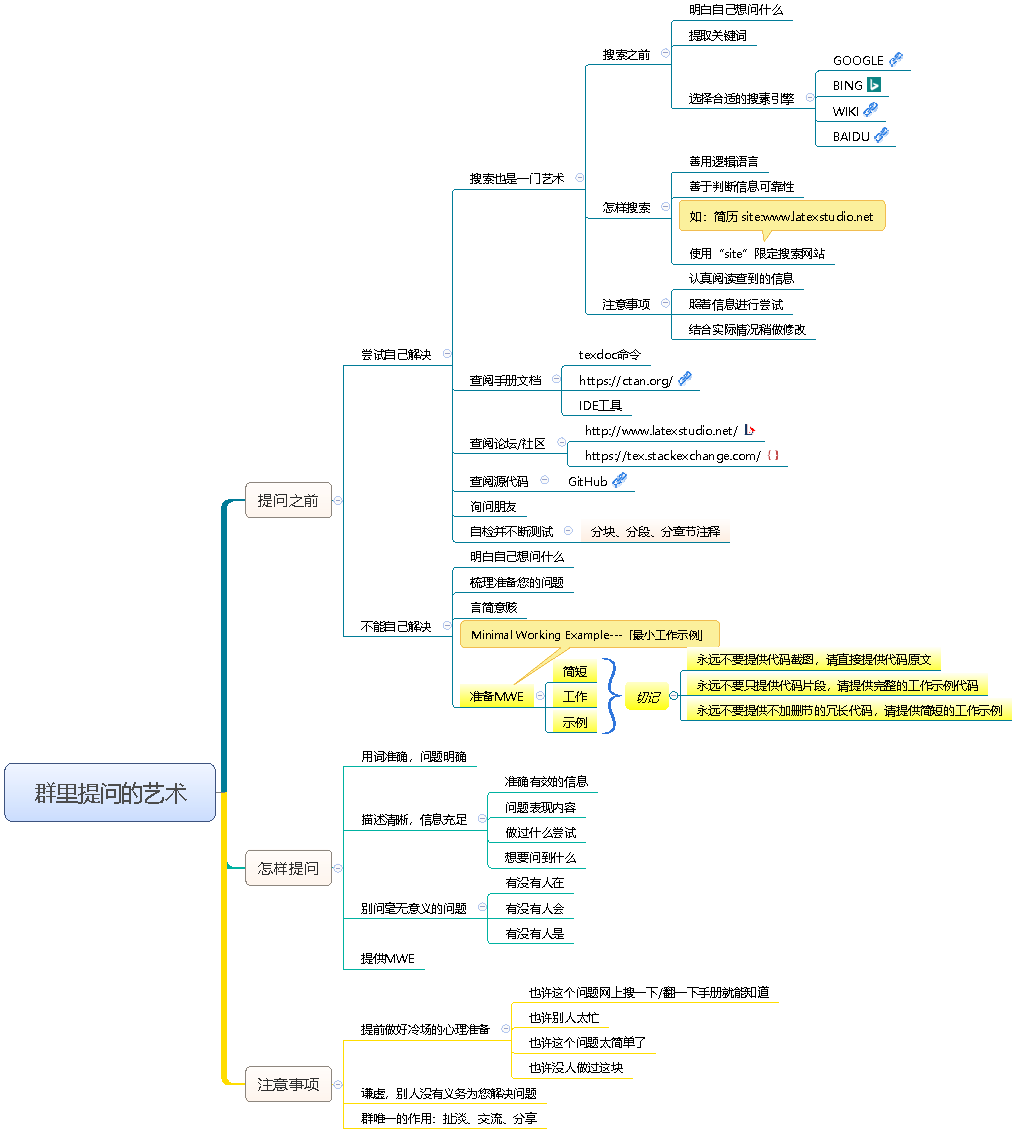
\includegraphics[width=0.45\textwidth]{smartqa}
  \stretchoff
\end{frame}

\begin{frame}{如何学\LaTeX ?}{提问的智慧}
  \stretchon
  \begin{itemize}
  \item 自力更生,艰苦奋斗\footnote[frame]{表情作者:龙茗安}    
  \end{itemize}
  \centering
  
\includegraphics[scale=1.6]{lma01}\\[4ex]
  
\includegraphics[scale=1.6]{lma02}
  \stretchoff
\end{frame}

\begin{frame}{如何学\LaTeX ?}{提问的智慧}
  \stretchon
  \begin{itemize}
  \item 提供\alert{MWE}---Minimum Work Example\footnote[frame]{\href{https://wenda.latexstudio.net/note/view/1.html}{https://wenda.latexstudio.net/note/view/1.html}。}    
  \end{itemize}
  \centering
  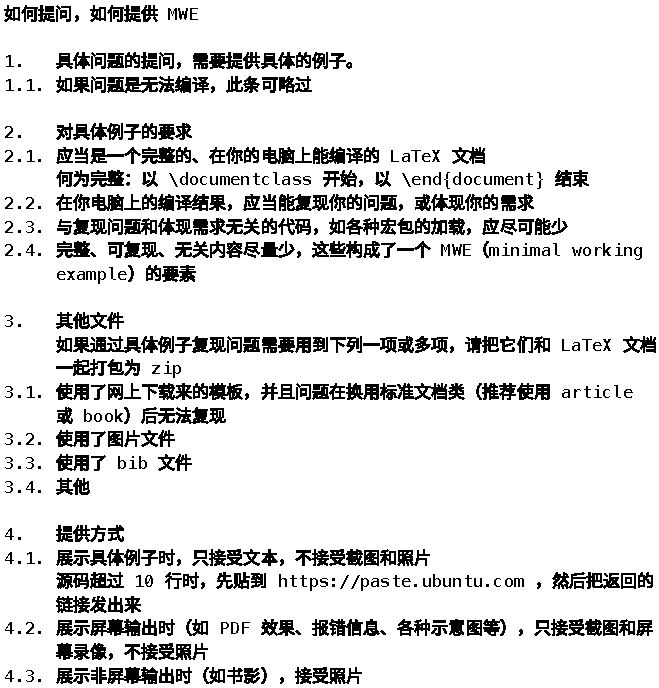
\includegraphics[width=0.45\textwidth]{mwe}
  \stretchoff
\end{frame}

\begin{frame}{如何学\LaTeX ?}{友情提醒}
  \stretchon
  \begin{itemize}
  \item 量力而行    
  \end{itemize}
  \centering
  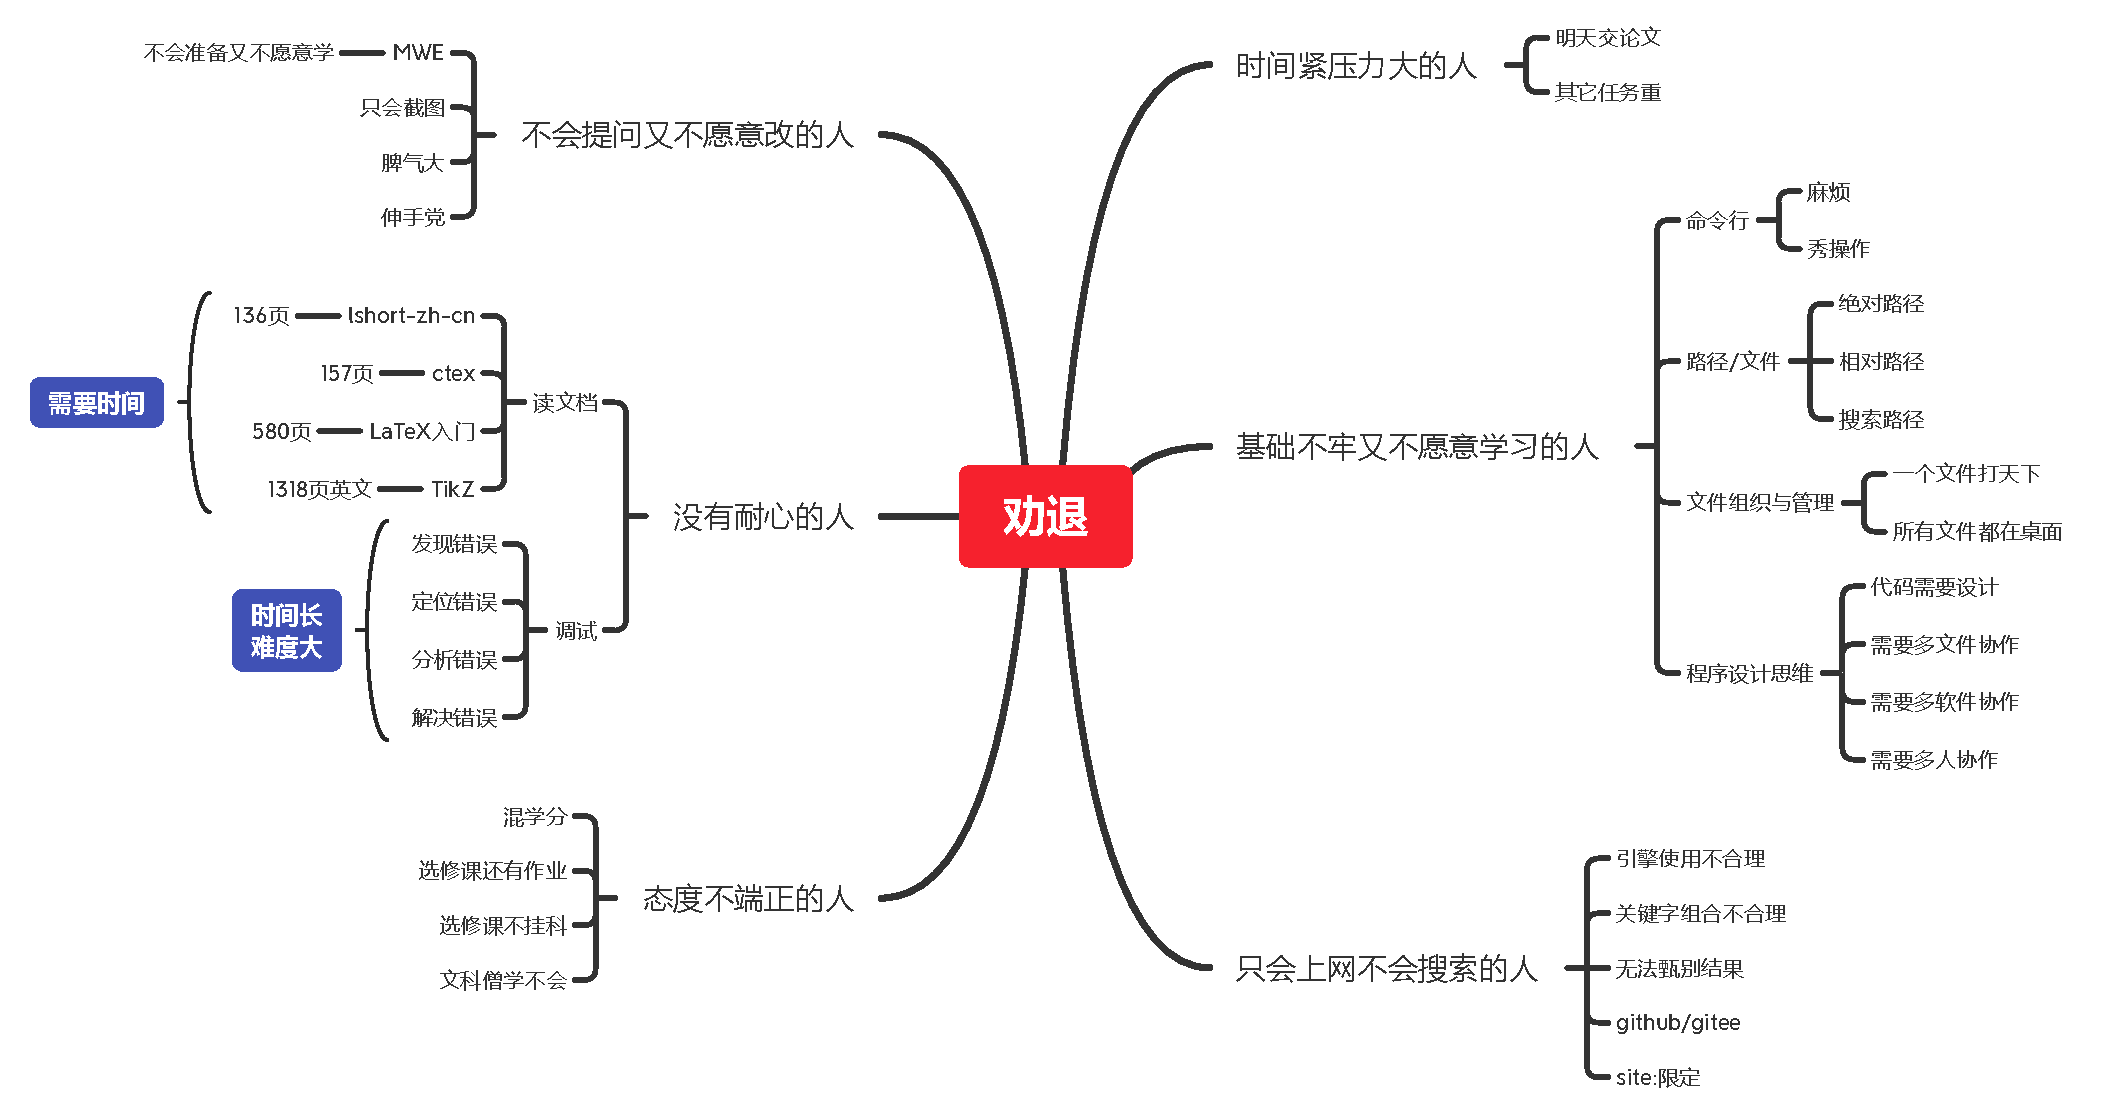
\includegraphics[height=0.8\textheight]{rejectlatex}
  \stretchoff
\end{frame}

\subsection[文档结构]{\latex 的文档结构}\label{sec02-02}
\begin{frame}{学习\LaTeX}{文档结构}
  \vspace{-4ex}
  \begin{spacing}{1.1}
  \begin{columns}
    \begin{column}{0.55\textwidth}
      
      \begin{itemize}
      \item {\only<2>{\color{red}}引入文档模板命令}\\
        \begin{itemize}
        \item {\only<2>{\color{red}}\textbackslash documentclass}
        \end{itemize}
      \item {\only<3>{\color{red}}导言区:} \par
        用于设置全局命令
        \begin{itemize}
        \item {\only<4>{\color{red}}宏包:} \par
          扩展基本\latex 命令
        \item {\only<5>{\color{red}} 定义/命令/宏:}\par
          用户自定义的命令
        \end{itemize}
      \item {\only<6>{\color{red}}文稿:}
        \begin{itemize}
        \item {\only<7>{\color{red}}命令:} \par
          影响参数内部或\{...\}区块中的文本  
        \item {\only<8>{\color{red}}环境:} \par
          只影响环境内部的文本
        \end{itemize}
      \end{itemize}
      
    \end{column}

    \begin{column}{0.35\textwidth}
      \begin{block}{.tex file}
        {
          \tiny \ttfamily
         {\only<2>{\color{red}} \textbackslash documentclass[letterpaper, 11pt]\{ctexart\}} \par
         {\only<3>{\color{red}}\% 导言区 \par          
          \quad {\only<4>{\color{red}} \% 宏包 \par
          \quad \textbackslash usepackage[margin=2.5cm]\{geometry\} \par
          \quad \textbackslash usepackage\{graphicx\} \par
          \quad ...} \par
         \quad {\only<5>{\color{red}} \% 自定义命令 \par
         \quad \textbackslash newcommand\{name\}[num]\{definition\} \par
         \quad ...}
       }\par
         
       \par
       {\only<6>{\color{red}} \% 文稿 \par
       \textbackslash begin\{document\} \par
       ... \par
       \quad {\only<7>{\color{red}}\textbackslash section\{...\}} \par
       \quad ... \par
       \qquad {\only<7>{\color{red}}\textbackslash subsection\{...\}} \par
       \qquad ... \par
       \quad \qquad {\only<8>{\color{red}}\textbackslash
       begin\{equation\} \par
       \quad \qquad ... \par
       \quad \qquad \textbackslash end\{equation\}} \par
       \qquad ... \par
       \quad {\only<7>{\color{red}}\textbackslash section\{...\}} \par
       ... \par
       \par
       \textbackslash end\{document\} \par
       } }
     \end{block}
   \end{column}
 \end{columns}
 \end{spacing}
\end{frame}

\begin{frame}[t, fragile]{学习\LaTeX}{命令和环境}
  \stretchon
  \begin{itemize}
  \item 文稿({\TeX}源文件)
    \begin{itemize}
    \item 正文
    \item 排版控制命令
    \end{itemize}
  \item 排版控制命令:用\alert{倒斜线}引导的字符串
    \begin{itemize}
    \item 控制字:一个或多个字母构成,区分大小写,如:\texinline{\alpha}
    \item 控制符:一个特殊字符构成,如\texinline{\%}
    \end{itemize}
  \item 排版命令的参数:\\
    \fbox{%
      \textbackslash {\color{blue}{排版命令}}[{\color{green}{可选参
          数}}]$\left\{\text{\color{red}{其它参数}}\right\}$ }%
    \begin{itemize}
    \item 方括号中的参数为可选
    \item 花括号中的其它参数是不可省略的参数
    \item 命令也可以不带参数
    \end{itemize}
  \item 环境: \texinline{\begin{xxx}}和\texinline{\end{xxx}}之间的内容
    \begin{itemize}
      \item \alert{一篇文章有且只能有一个\texinline{document}环境}
    \end{itemize}
  \end{itemize}
  \stretchoff
\end{frame}

\begin{frame}[t,fragile]{学习\LaTeX}{基本约定}
  \stretchon
  \begin{itemize}
  \item 分组:\{ $\cdots\cdots$ \}
    \begin{itemize}
    \item 欢迎你来到{\latex}(\verb|{\LaTeX}|)世界,
    \end{itemize}
  \item 注释:\%开始的一行
  \item 西文标点后要加空格
  \item 建议各种环境的开始和结束各占一行
  \item 多个空格算1个空格
  \item \alert{换行分段}:1个回车仅视为1个空格,2个以上回车视为1个换行
  \end{itemize}
  \stretchoff
\end{frame}

\subsection{处理错误}
\begin{frame}[t, fragile]{常见错误}{命令未定义}
  \stretchon
  \begin{itemize}
  \item 命令名称\alert{输入}错误\\[3ex]
  
  
  如将 \texinline{\author{作者}} 写为 \texinline{\authos{作者}},
  编译后会看到如下错误信息:
  \begin{texcode}
    ! Undefined control sequence.
    l.12 \authos
  \end{texcode}
  其中:
  \begin{itemize}
  \item 第一行说明错误原因是“命令未定义”
  \item 第二行说明错误出现在第 12行的 \texinline{\authos} 这里。
  \end{itemize}
  
  \end{itemize}
  \stretchoff
\end{frame}

\begin{frame}[t, fragile]{常见错误}{缺少\$ 、\$\$等符号}
  \stretchon
  \begin{itemize}
  \item 例如缺少\$号\\[3ex]
  
  
    第二常见的错误是忘记将公式放在一对\qtmark{\$} 里,如:

    将 \texinline{$2^3=8$} 错写为 \texinline{2^3=8},
  编译后将会看到如下错误信息:
  \begin{texcode}
    ! Missing $ inserted.
    <inserted text>
                    $
    l.19 2^
           3=8
  \end{texcode}
  其中:
  \begin{itemize}
  \item 第一行说明错误原因是“缺少\$号”,
  \item 后面几行说明错误出现在第 19行的 \texinline{2^3=8} 这里。
  \end{itemize}
  
  \end{itemize}
  \stretchoff
\end{frame}

\begin{frame}[t, fragile]{常见错误}{括号不配对}
  \stretchon
  \begin{itemize}
  \item 例如花括号\}不配对\\[3ex]
  
  
    第三常见的错误是花括号无法配对,如:

    将根号 \texinline!$\sqrt{2}$! 错写为 \texinline!$\sqrt{2]$!,
  编译后将会看到如下错误信息:
  \begin{texcode}
    ! Missing } inserted.
    <inserted text>
                    }
    l.17 $\sqrt{2]$
  \end{texcode}
  其中:
  \begin{itemize}
  \item 第一行说明错误原因是“缺少 \} 号”
  \item 后面几行说明错误出现在第 17 行这里。
  \end{itemize}
  
  \end{itemize}
  \stretchoff  
\end{frame}

\section[\nwafuprojrep]{\nwafuprojrep() 实习报告/论文模板简介}
\subsection[开发需求]{开发需求}
\begin{frame}[t]{\nwafuprojrep 模板}{开发需求}
  \stretchon
  \begin{itemize}
  \item 西北农林科技大学信息工程学院实习报告/论文撰写规定
  \end{itemize}
  \centering
  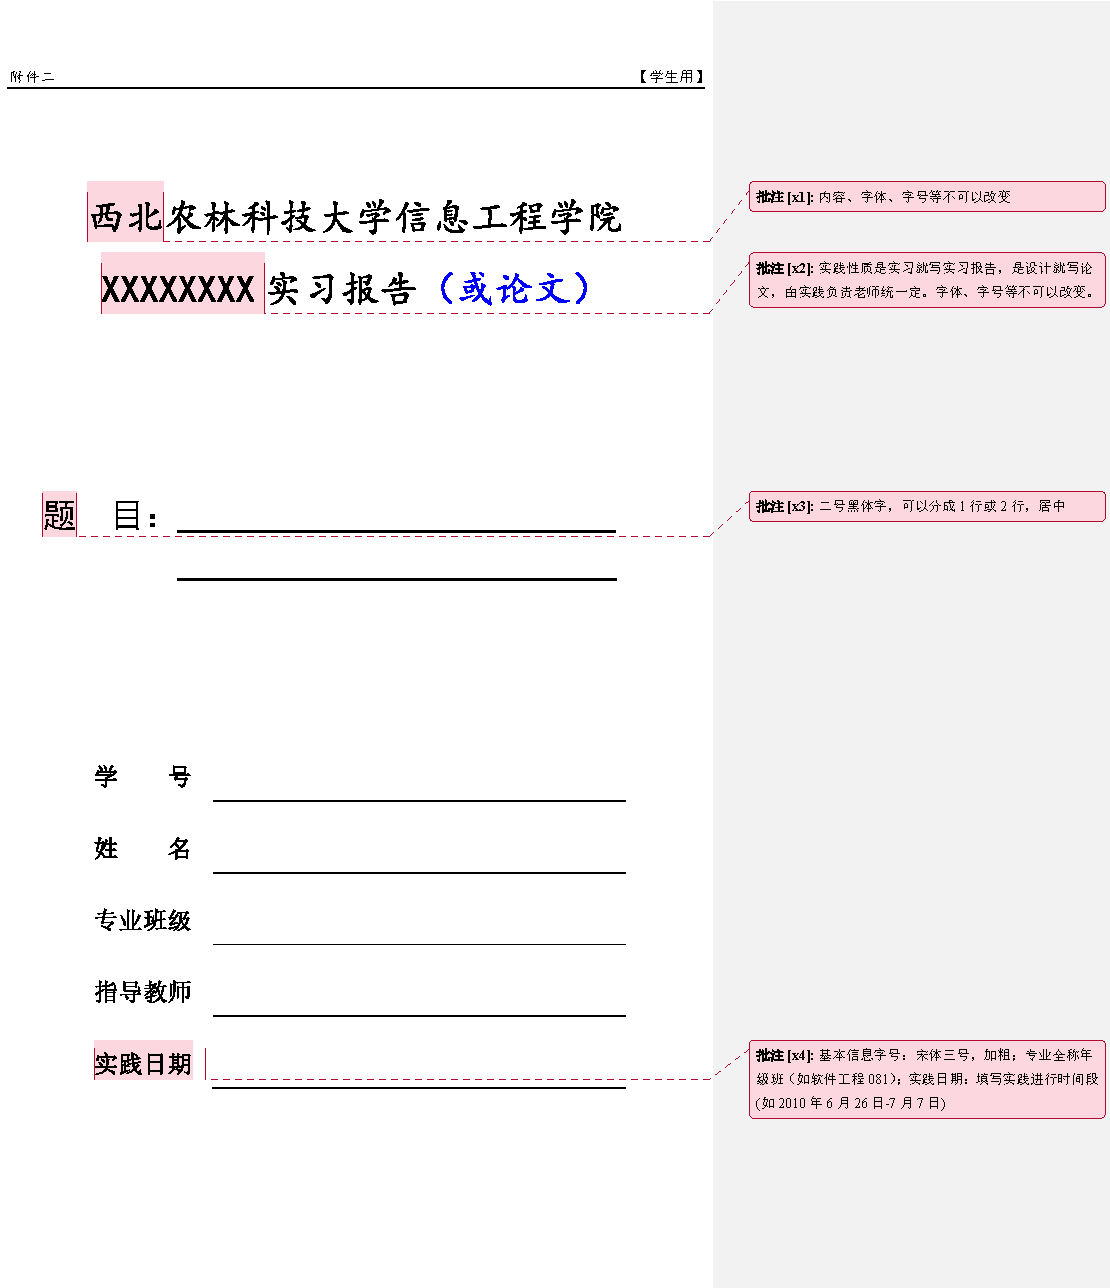
\includegraphics[height=0.7\textheight]{projrep01}\qquad
  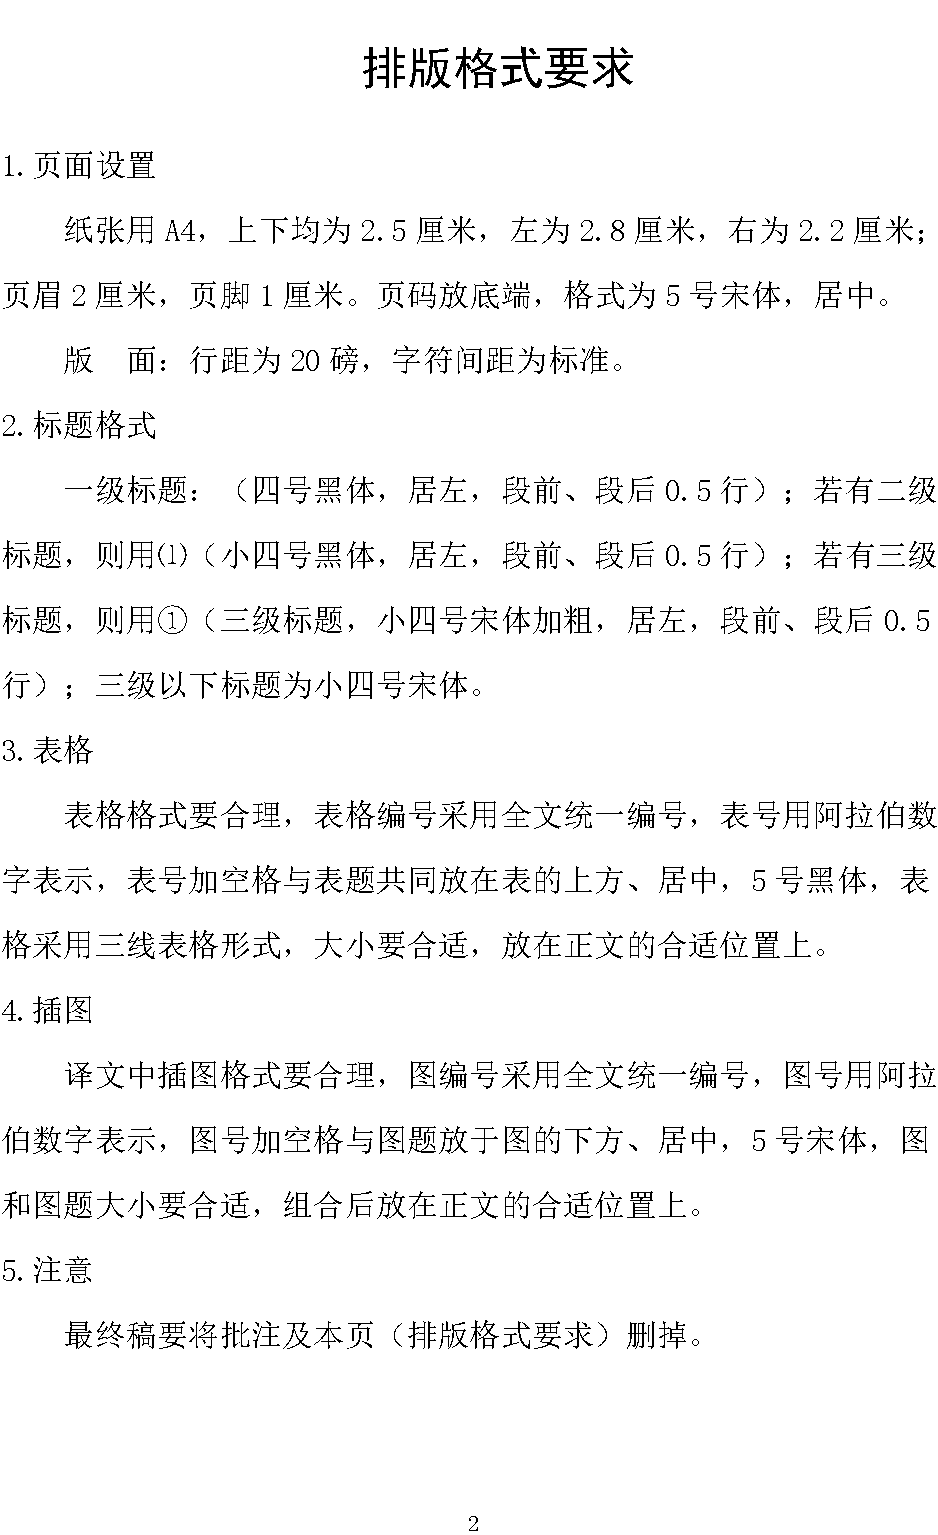
\includegraphics[height=0.7\textheight]{projrep02}
  \stretchoff
\end{frame}

\subsection[模板下载]{模板下载}
\begin{frame}[t]{\nwafuprojrep 模板}{模板下载}
  \stretchon
  \begin{itemize}
  \item \faGithub
    Gitee\link{https://gitee.com/registor/nwafuprojrep}{(\alert{推
        荐})}\footnote[frame, 1]{问题反馈、实时更新等Gitee发布。}\footnote[frame, 2]{湿兄用U盘拷给你的模板一定是过时的。}
    \begin{itemize}
    \item 模板必须文件
      \begin{itemize}
      \item \LaTeX 文档类(模板): \qtmark{nwafuprojrep.cls}
      \end{itemize}
    \item release 打包下载(含样例及模板所需文件)
    \end{itemize}
  \end{itemize}
  \stretchoff
\end{frame}

\subsection[模板使用]{模板使用}
\begin{frame}[fragile]{\nwafuprojrep 模板}{模板使用}
  %\stretchon
  \begin{itemize}  
  \item 用\texinline{\documentclass{nwafuprojrep}}引入文档类(模板)\footnote[frame, 1]{看文档、看文档、看文档}
    \begin{itemize}
    \item 用可选参数指定论文类型---报告或论文,默认是报告
    \item 用可选参数指定输出类型---打印或电子稿,默认是电子稿
    \end{itemize} 
  \item 用\texinline{\nwafuset}命令设置中文题目、作者、导师等基本数据
  %\end{itemize}
  %\vspace{-1ex}
  \begin{center}
    \begin{minipage}[h]{0.75\linewidth}
      \texfile[fontsize=\zihao{8}]{code/nwafuset.tex}  
    \end{minipage}
  \end{center}\vspace{-3ex}
  %\begin{itemize}  
  \item 撰写报告或论文
  \end{itemize}
  %\stretchoff
\end{frame}

\begin{frame}[t]{\nwafuprojrep 模板}{模板使用}
  \stretchon
  \begin{spacing}{1.8}  
  \begin{itemize}  
  \item 撰写论文
    \begin{itemize}
    \item 直接撰写
    \item 改写样例(\alert{推荐})
    \end{itemize}
  \item 注意事项
    \begin{itemize}
    \item 文件及路径名不用中文和空格
    \item 坚持\alert{内容与格式的分离}思想
    \end{itemize}
  \end{itemize}
  \end{spacing}
  \stretchoff
\end{frame}

\subsection[注意事项]{注意事项}
\begin{frame}[t]{\nwafuprojrep 模板}{注意事项}
  \stretchon
  \begin{itemize}
  \item 基本原则:\alert{内容与格式分离}
  \item 正确(或曰:合理)的做法

    \begin{itemize}
      \item 强调文字(加粗):\texinline{\emph{...}}
      \item 摘要(居中,小字号,带有标题):\texinline{abstract} 环境
      \item 个人简历:\texinline{resume}环境
      \item $\cdots\cdots$  
      \item 自定义新的命令、环境
    \end{itemize}

  \item 记得学会\alert{偷懒!}
    
  \end{itemize}
  \stretchoff
\end{frame}

\begin{frame}[fragile]{\nwafuprojrep 模板}{注意事项}
  %\stretchon
  \begin{itemize}
  \item 浮动体与交叉引用
    \begin{itemize}
    \item 浮动体机制
      \begin{itemize}
      \item \texinline{figure} 和 \texinline{table} 环境
      \item 图、表浮动(乱跑)不是BUG,是\LaTeX 的精髓!
      \item 希望浮动体不要乱跑:\alert{「这是病,得治」}\link{https://liam.page/2017/03/11/floats-in-LaTeX-basic}
      \item 避免「见上图」、「见下表」
      \end{itemize}
    \item 浮动参数
      \begin{itemize}
      \item h(就摆这里)、t(页面顶端)、b(页面底端)、p(只有浮动体的页面)
      \item ! 求你了,听听我的请求吧……
      \end{itemize}
    \end{itemize}
  \end{itemize}
  \vspace{-1.5ex}
  \begin{center}
  \begin{minipage}[h]{0.35\linewidth}
    \begin{texcode}
      \begin{figure}[htb!]
        \includegraphics[...]{...}
        \caption{一个校徽}
        \label{fig:logo}
      \end{figure}
    \end{texcode}
  \end{minipage}\quad
  \begin{minipage}[h]{0.53\linewidth}
    \begin{texcode}
      \begin{table}[htb]
        \bicaption[...]{...\label{tab:bicap}}{...}
        \begin{tabular}{lr}
        \toprule
        城市 & 人口 \\
        \midrule
        Mexico City & 20,116,842\\
        \bottomrule
        \end{tabular}
      \end{table}
    \end{texcode}
  \end{minipage}
  \end{center}
  %\stretchoff
\end{frame}

\begin{frame}{\nwafuprojrep 模板}{注意事项}
  \stretchon
  \begin{itemize}
  \item 浮动体与交叉引用
    \begin{itemize}
    \item \alert{标签}控制交叉引用
      \begin{itemize}
      \item 被引处打标签:\texinline{\label}
      \item 引用处用标签:\alert{\texinline{\autoref}}、\texinline{\ref}、
        \texinline{\eqref}等
      \item 用有意义的标签:\texinline{\label{eq:euler-lagrange-eq}}
      \end{itemize}
    \item 文献\alert{键值}交叉引用
      \begin{itemize}
      \item 在文献数据库中(\pkg{*.bib})为每篇文献指定\alert{键值}(第1字段)
      \item 引用处用键值:\texinline{\textcite{键值}}、\texinline{\cite{键值}}系列命令引用文献
      \item 文献排版引擎:\pkg{biblatex} 宏包 + \pkg{biber} 后端
      \item 模板已设置,\alert{无需更改}
      \end{itemize} 
    \item 需多次编译---推荐 \pkg{latexmk}      
    \end{itemize}
  \end{itemize}  
  \stretchoff
\end{frame}

\begin{frame}{\nwafuprojrep 模板}{注意事项}
  \stretchon
  \begin{itemize}
  \item 插图
    \begin{itemize}
    \item 外部插入

      \begin{itemize}
      \item Mathematica、MATLAB
      \item PowerPoint、Visio、Adobe Illustrator、Inkscape
      \item Python Matplotlib、\texttt{Plots.jl}、R、Plotly
      \item $\cdots\cdots$
      \end{itemize}

    \item \TeX{} 内联绘图

      \begin{itemize}
      \item Asymptote
      \item \alert{\pkg{pgf}/\pkg{TikZ}、\pkg{pgfplots}}
      \end{itemize}

    \item 插图格式

      \begin{itemize}
      \item 矢量图:\texttt{.pdf}(\alert{强烈推荐})
      \item 位图:\texttt{.jpg} 或 \texttt{.png}
      \item \alert{不再推荐 \texttt{.eps}}
      \item 不(完全)支持 \texttt{.svg}、\texttt{.bmp}
      \end{itemize}
    \end{itemize}
  \end{itemize}
  \stretchoff
\end{frame}

\begin{frame}{\nwafuprojrep 模板}{注意事项}
  \stretchon
  \begin{itemize}
  \item 文献数据库(\pkg{*bib})
    \begin{itemize}
    \item 建议自动生成 (你只有三篇参考文献?)
      \begin{itemize}
      \item \href{http://xueshu.baidu.com/}{百度学术}、Google Scholar等可直接复制
      \end{itemize}
      
    \end{itemize}
  \end{itemize}
  \centering
  \begin{annotatedFigure}
    {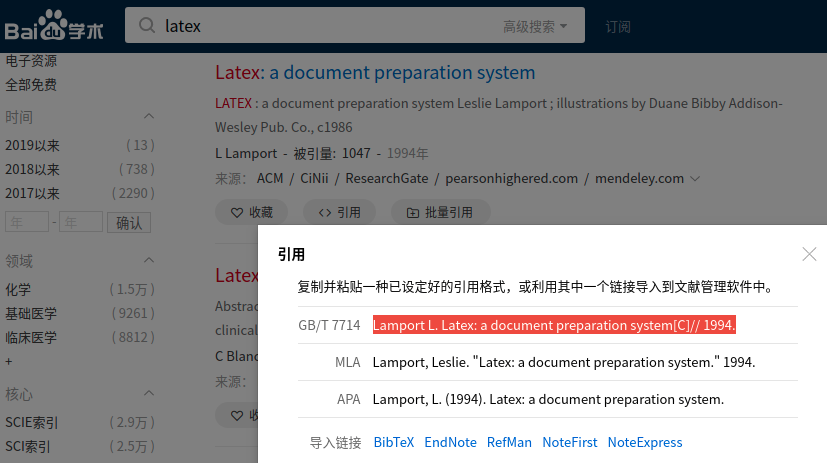
\includegraphics[width=0.4\textwidth]{baiduxueshu}}
    \annotatedFigureBox{0.36,0.51}{0.46,0.58}{red}
    \annotatedFigureBox{0.44,0.015}{0.51,0.08}{blue}
  \end{annotatedFigure}\quad
  \begin{annotatedFigure}
    {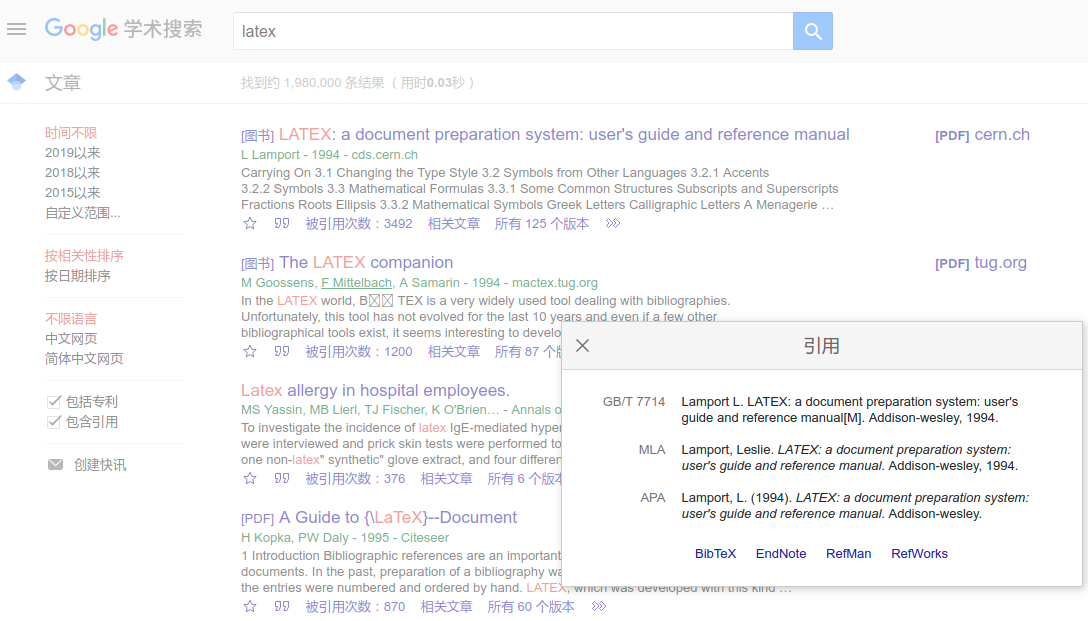
\includegraphics[width=0.4\textwidth]{googlescholar}}
    \annotatedFigureBox{0.24,0.62}{0.28,0.66}{red}
    \annotatedFigureBox{0.63,0.08}{0.685,0.14}{blue}
  \end{annotatedFigure}\\[2ex]
  \begin{annotatedFigure}
    {
\includegraphics[width=0.4\textwidth]{baiduxueshu-bibtex}}
    \annotatedFigureBox{0.005,0.05}{0.96,0.55}{blue}
  \end{annotatedFigure}
  \stretchoff
\end{frame}

\begin{frame}{\nwafuprojrep 模板}{注意事项}
  %\stretchon
  \begin{itemize}
  \item 文献数据库(\pkg{*bib})
    \begin{itemize}
    \item 建议自动生成 (你只有三篇参考文献?)

      \begin{itemize}
      \item 用Zotero\footnote[frame,1]{在此,以知网为例,适合所有网站。}、Jabref、NoteExpress等软件辅助
      \end{itemize}
      
    \end{itemize}
  \end{itemize}
  \centering
  \vspace{6ex}
  \begin{annotatedFigure}
    {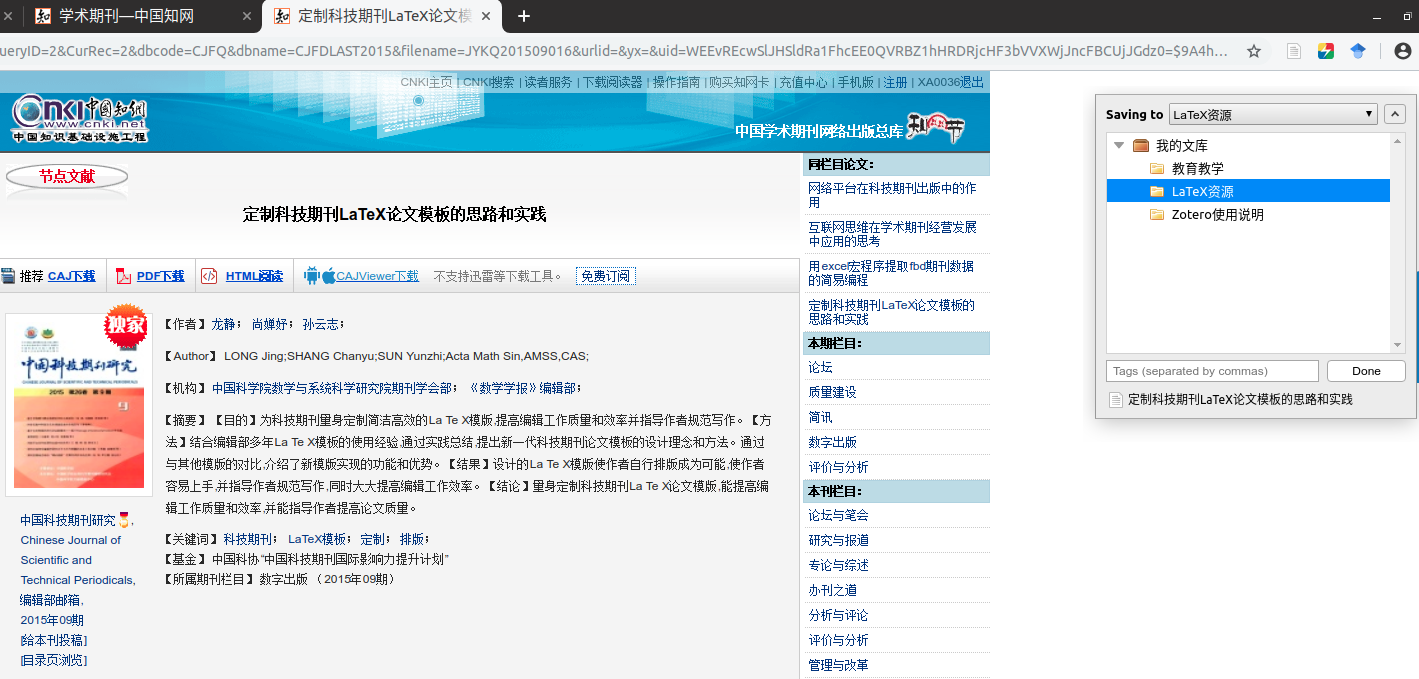
\includegraphics[height=0.365\textheight]{zotero-conect}}
    \annotatedFigureBox{0.895,0.9}{0.925,0.95}{red}
    \annotatedFigureBox{0.77,0.38}{0.995,0.86}{blue}
  \end{annotatedFigure}\quad%\\%[2ex]
  \begin{annotatedFigure}
    {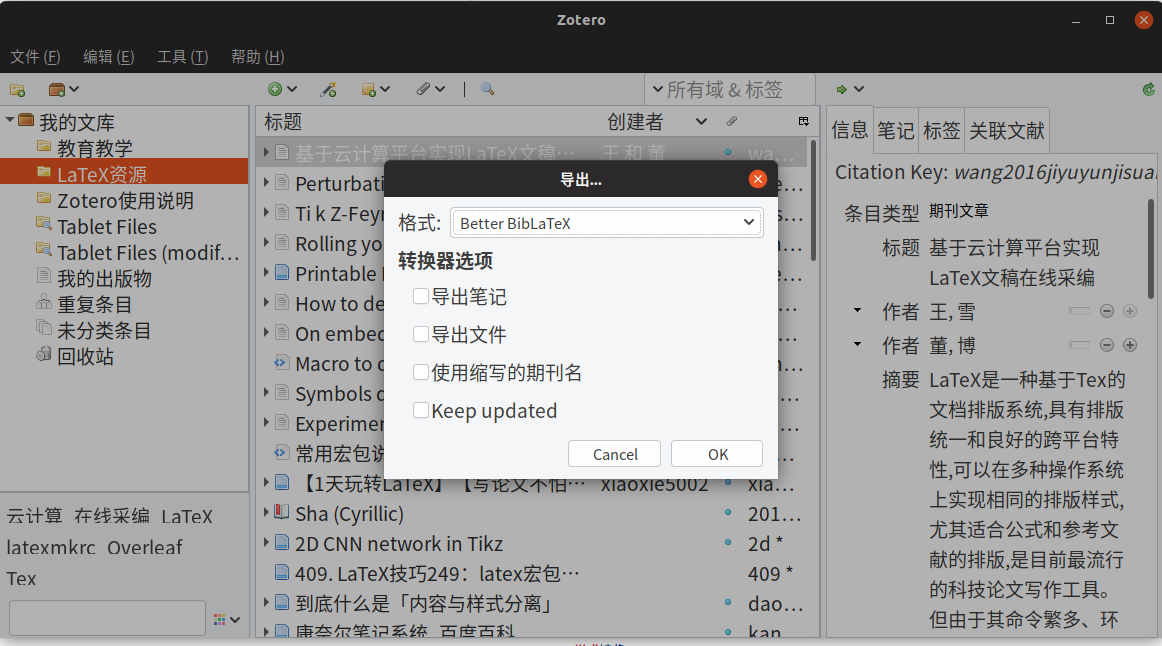
\includegraphics[height=0.365\textheight]{zotero}}
    \annotatedFigureBox{0.33,0.263}{0.67,0.75}{blue}
  \end{annotatedFigure}
  %\stretchoff
\end{frame}

\subsection[TeXstudio]{TeXstudio配置}
\begin{frame}{\nwafuprojrep 模板}{TeXstudio配置}
  \stretchon
  \begin{itemize}
  \item 用\XeLaTeX \alert{4次}编译
    \begin{itemize}
    \item \menu[,]{选项,设置TeXstudio...,命令}
    \item 根据需要选择使用\texttt{-shell-escape}参数
    \end{itemize}
  \end{itemize}
  \centering
  \begin{annotatedFigure}
    {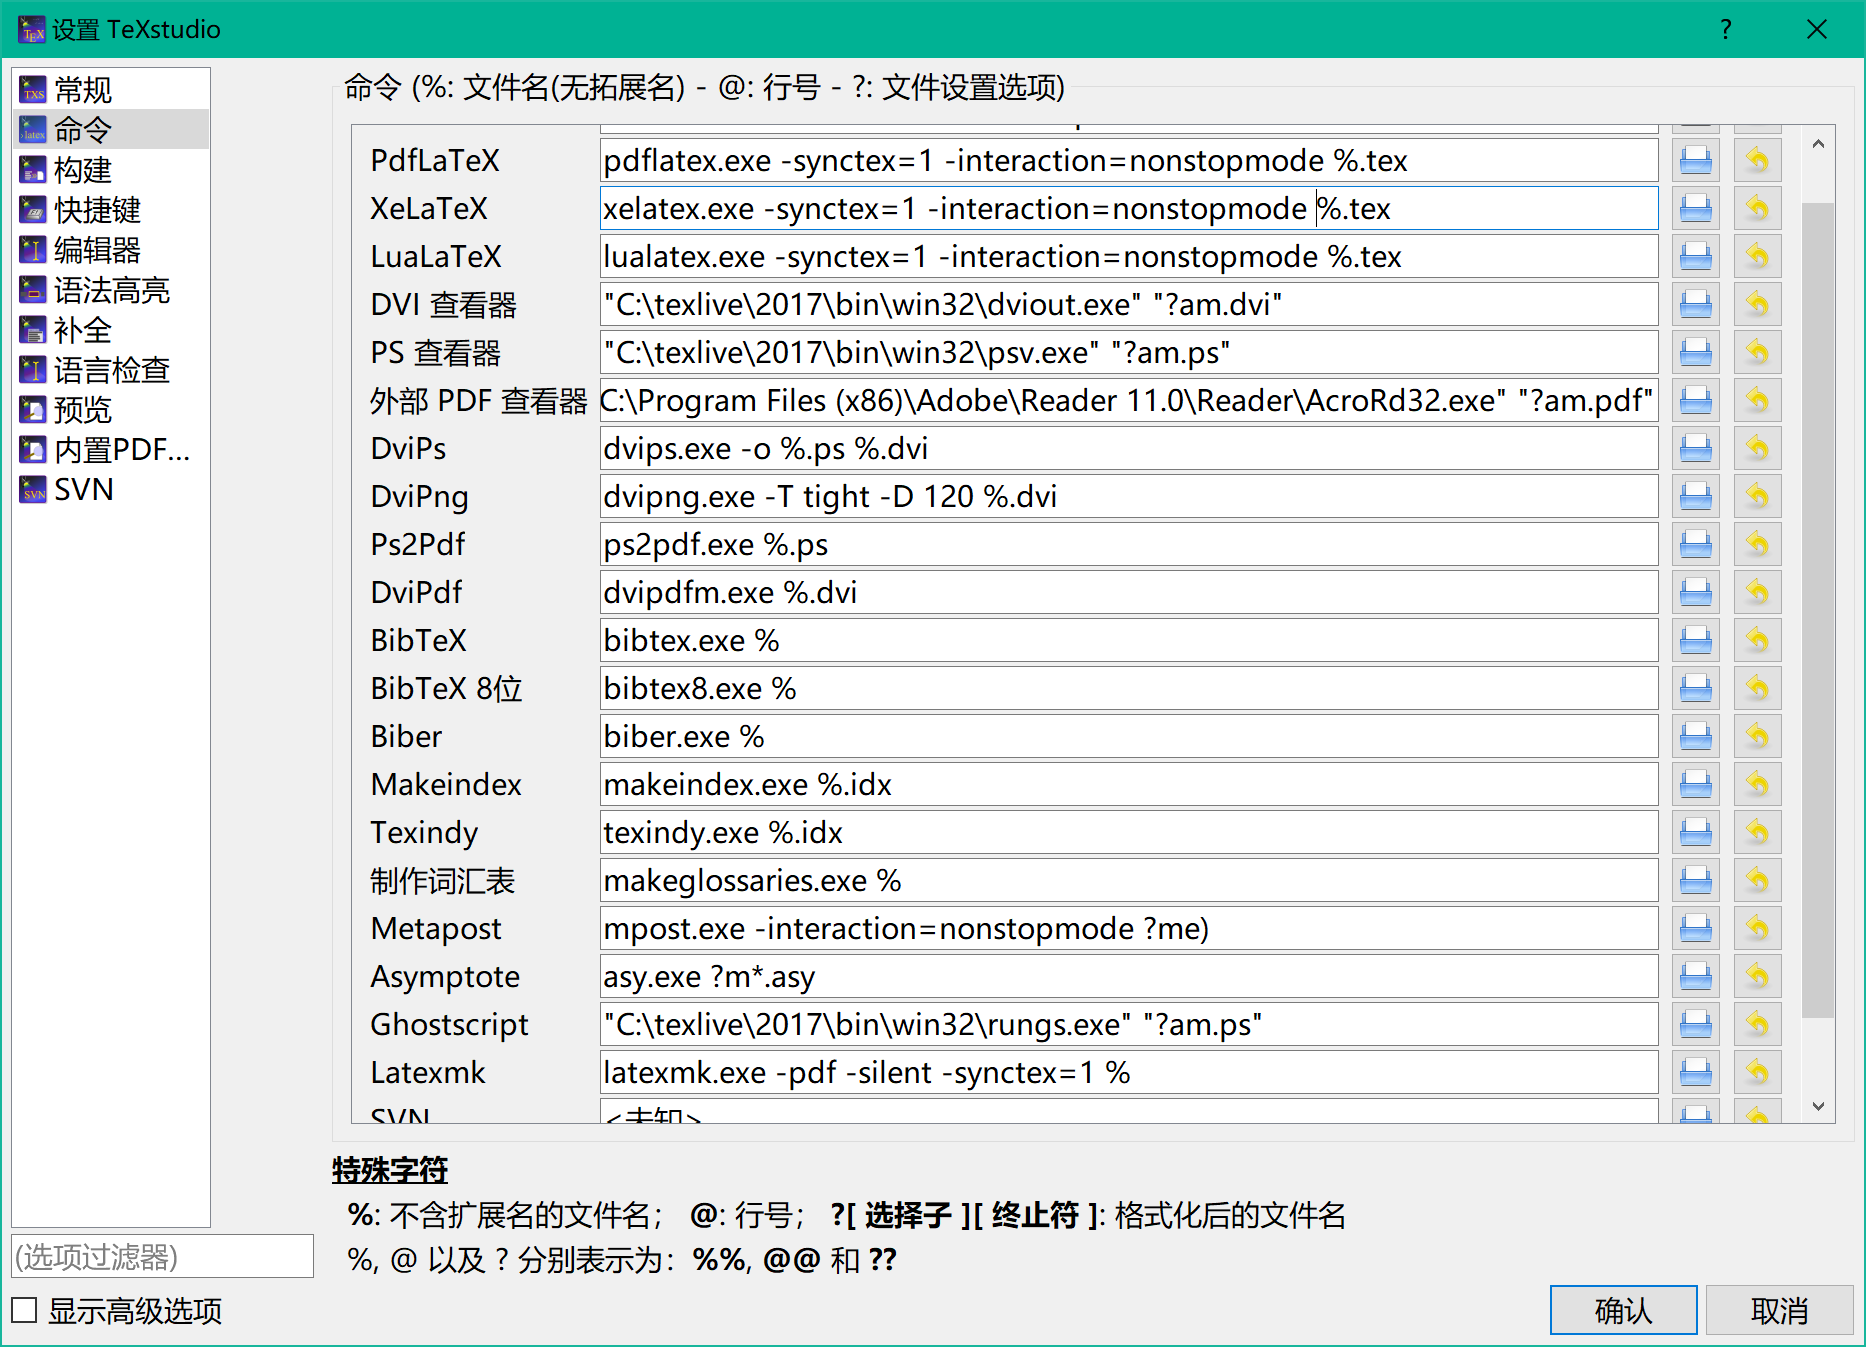
\includegraphics[width=0.45\textwidth]{texstudio-options-cmd-xelatex}}
    \annotatedFigureBox{0.005,0.88}{0.08,0.92}{red}
    \annotatedFigureBox{0.18,0.82}{0.8,0.87}{red}
  \end{annotatedFigure}
  \begin{annotatedFigure}
    {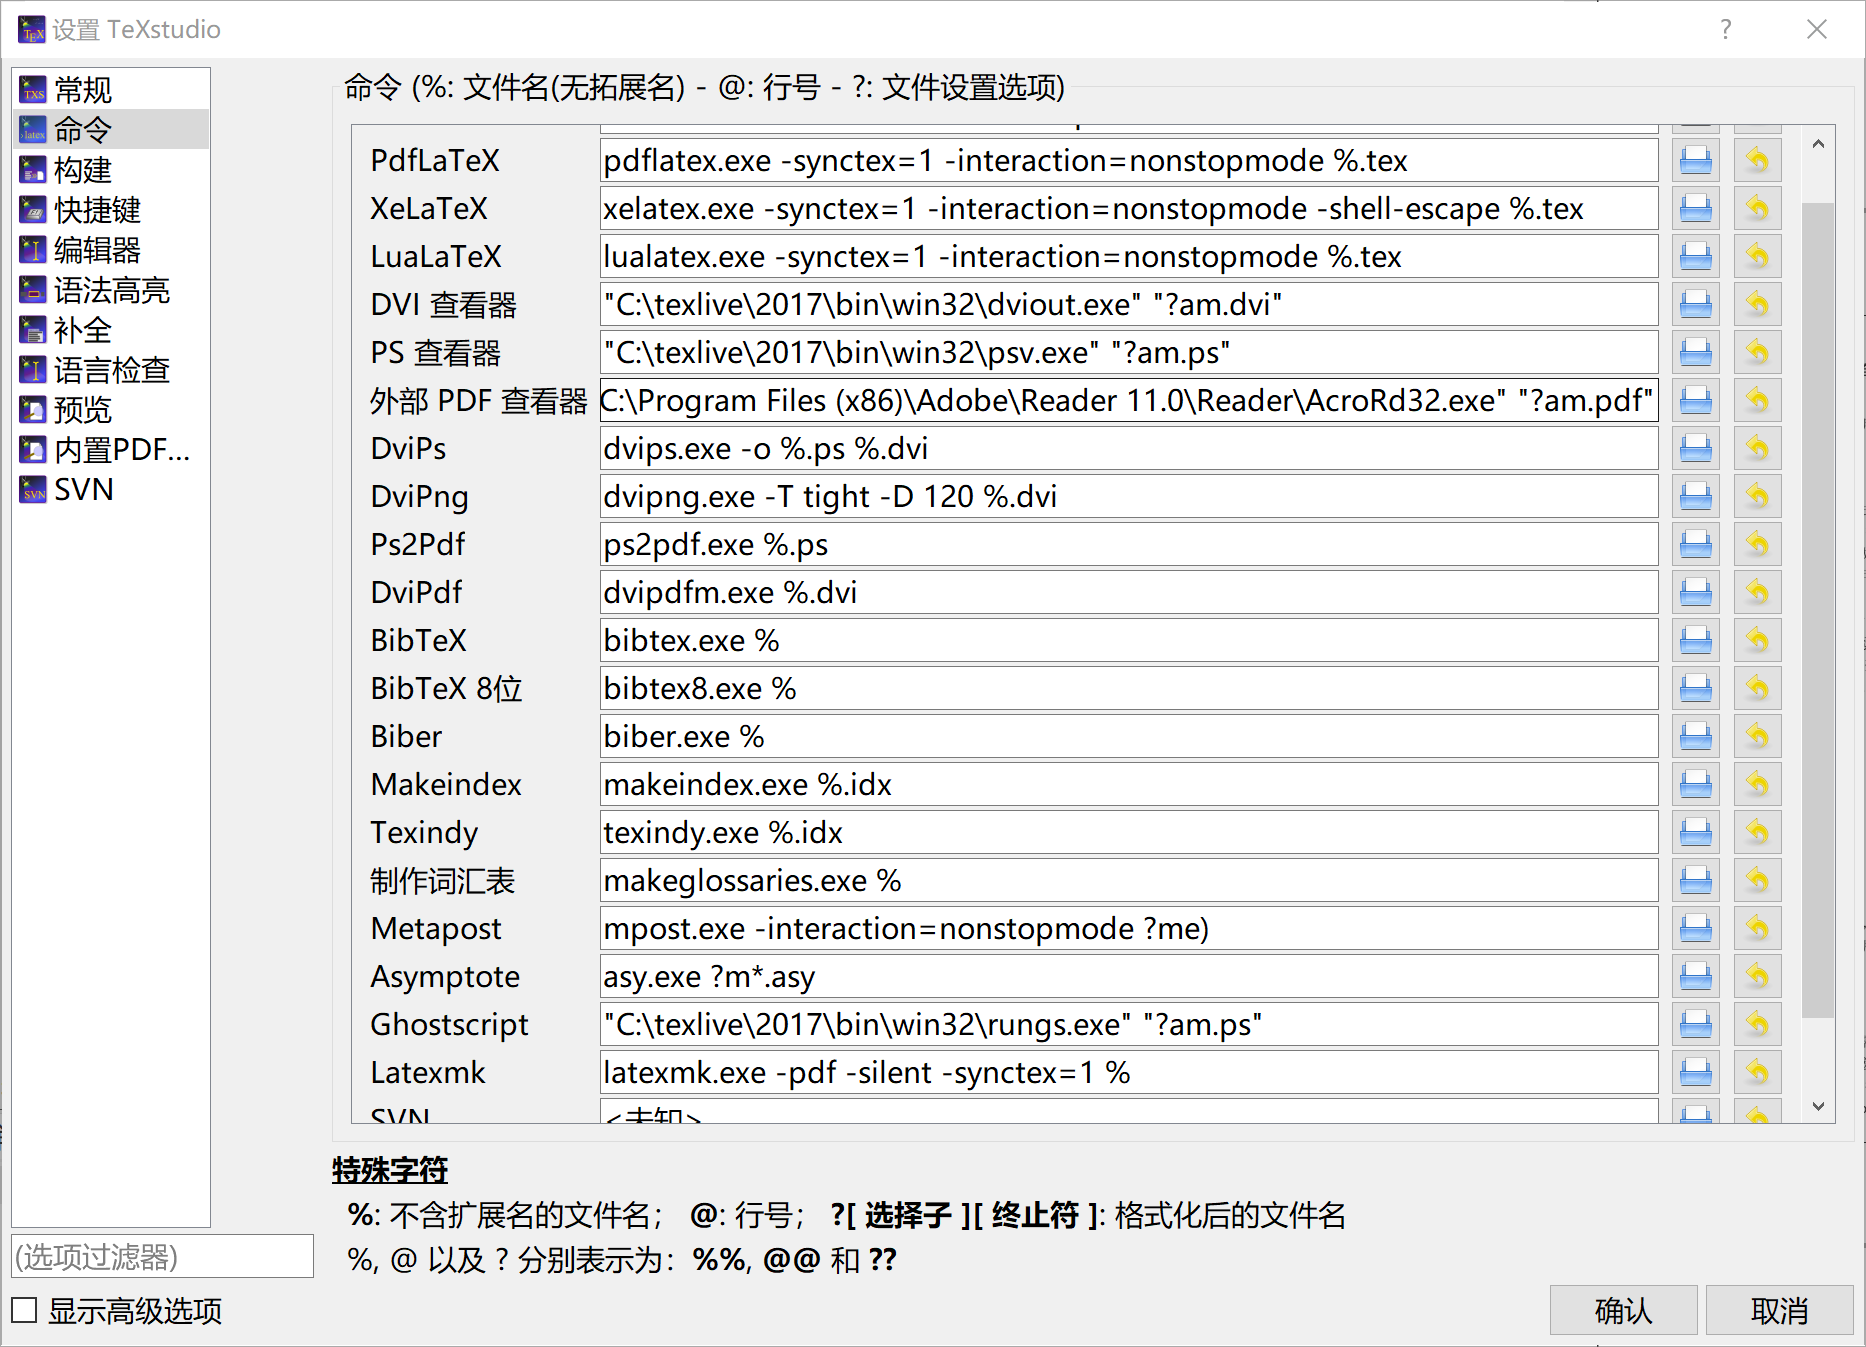
\includegraphics[width=0.45\textwidth]{texstudio-options-cmd-xelatex-withminted}}
    \annotatedFigureBox{0.68,0.82}{0.82,0.87}{blue}
  \end{annotatedFigure}  
  \stretchoff
\end{frame}

\begin{frame}{\nwafuprojrep 模板}{TeXstudio配置}
  \stretchon
  \begin{itemize}
  \item 用\XeLaTeX \alert{4次}编译
    \begin{enumerate}
    \item \XeLaTeX 编译\TeX 源码:\menu[,]{工具,构建并查看/F5}或
      \menu[,]{工具,编译/F6}\footnote[frame,1]{实践观察,点选一次菜单,
        则执行两次编译,如果有出入,请多执行几次。}
    \item Biber 编译参考文献:\menu[,]{工具,参考文献/F8}
    \item \XeLaTeX 编译\TeX 源码:\menu[,]{工具,构建并查看/F5}或 \menu[,]{工具,编译/F6}
    %\item \XeLaTeX 编译\TeX 源码:\menu[,]{工具,构建并查看/F5}或\menu[,]{工具,编译/F6}
    \end{enumerate}
  \end{itemize}
  \centering
  \begin{annotatedFigure}
    {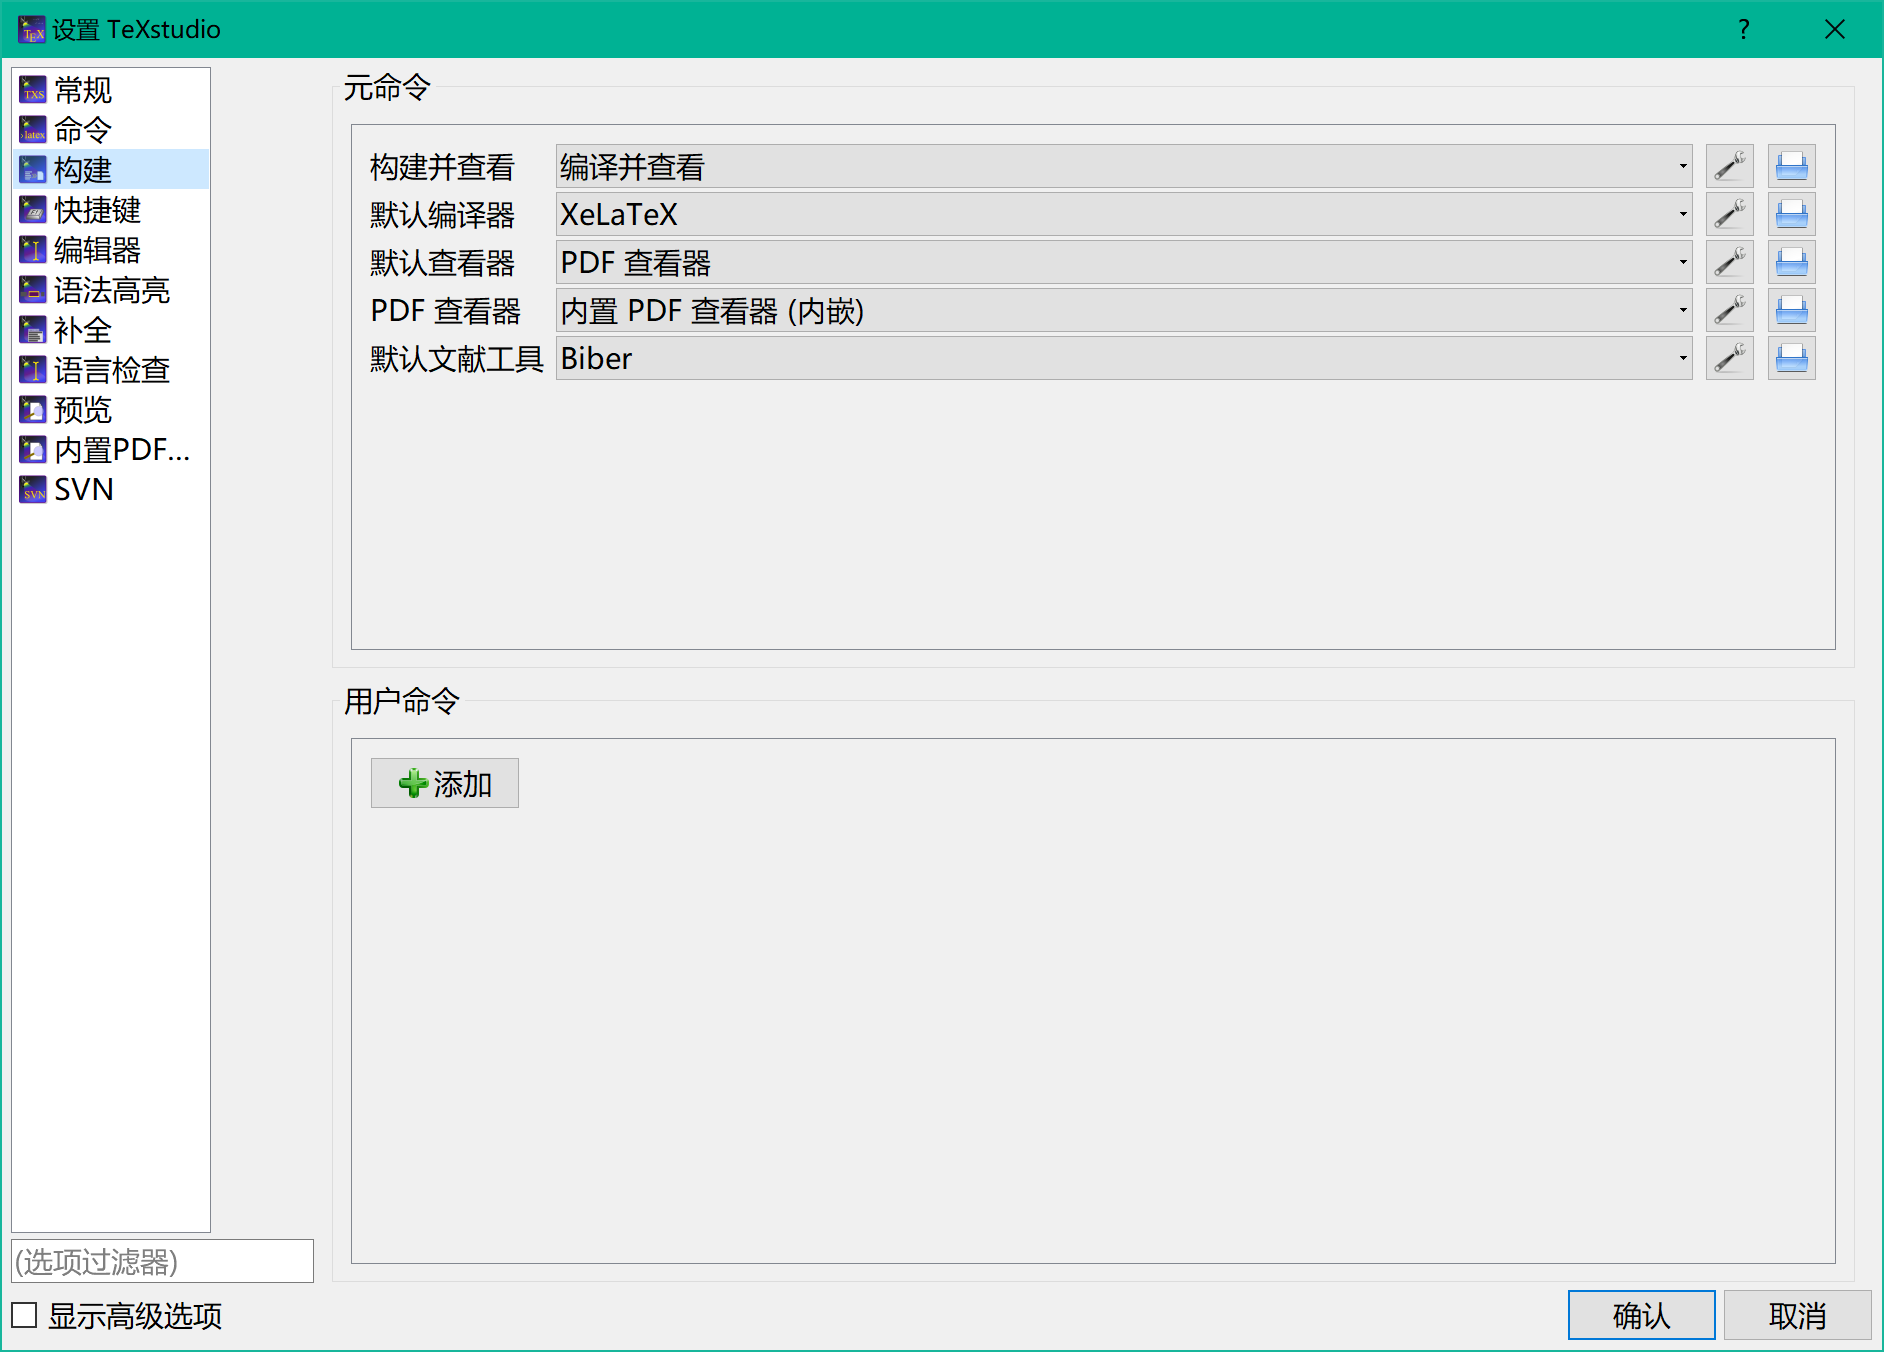
\includegraphics[width=0.45\textwidth]{texstudio-options-build-toolchains-xelatex-biber}}
    \annotatedFigureBox{0.005,0.855}{0.08,0.895}{red}
    \annotatedFigureBox{0.18,0.82}{0.4,0.86}{blue}
    \annotatedFigureBox{0.18,0.715}{0.4,0.755}{blue}
  \end{annotatedFigure}
  \stretchoff
\end{frame}

\begin{frame}{\nwafuprojrep 模板}{TeXstudio配置}
  \stretchon
  \begin{itemize}
  \item 用\pkg{latexmk} \alert{1次}编译
    \begin{itemize}
    \item 菜单:\menu[,]{选项,设置TeXstudio...,命令}
    \item 根据需要选择使用\texttt{-shell-escape}参数
    \end{itemize}
  \end{itemize}
  \centering
  \begin{annotatedFigure}
    {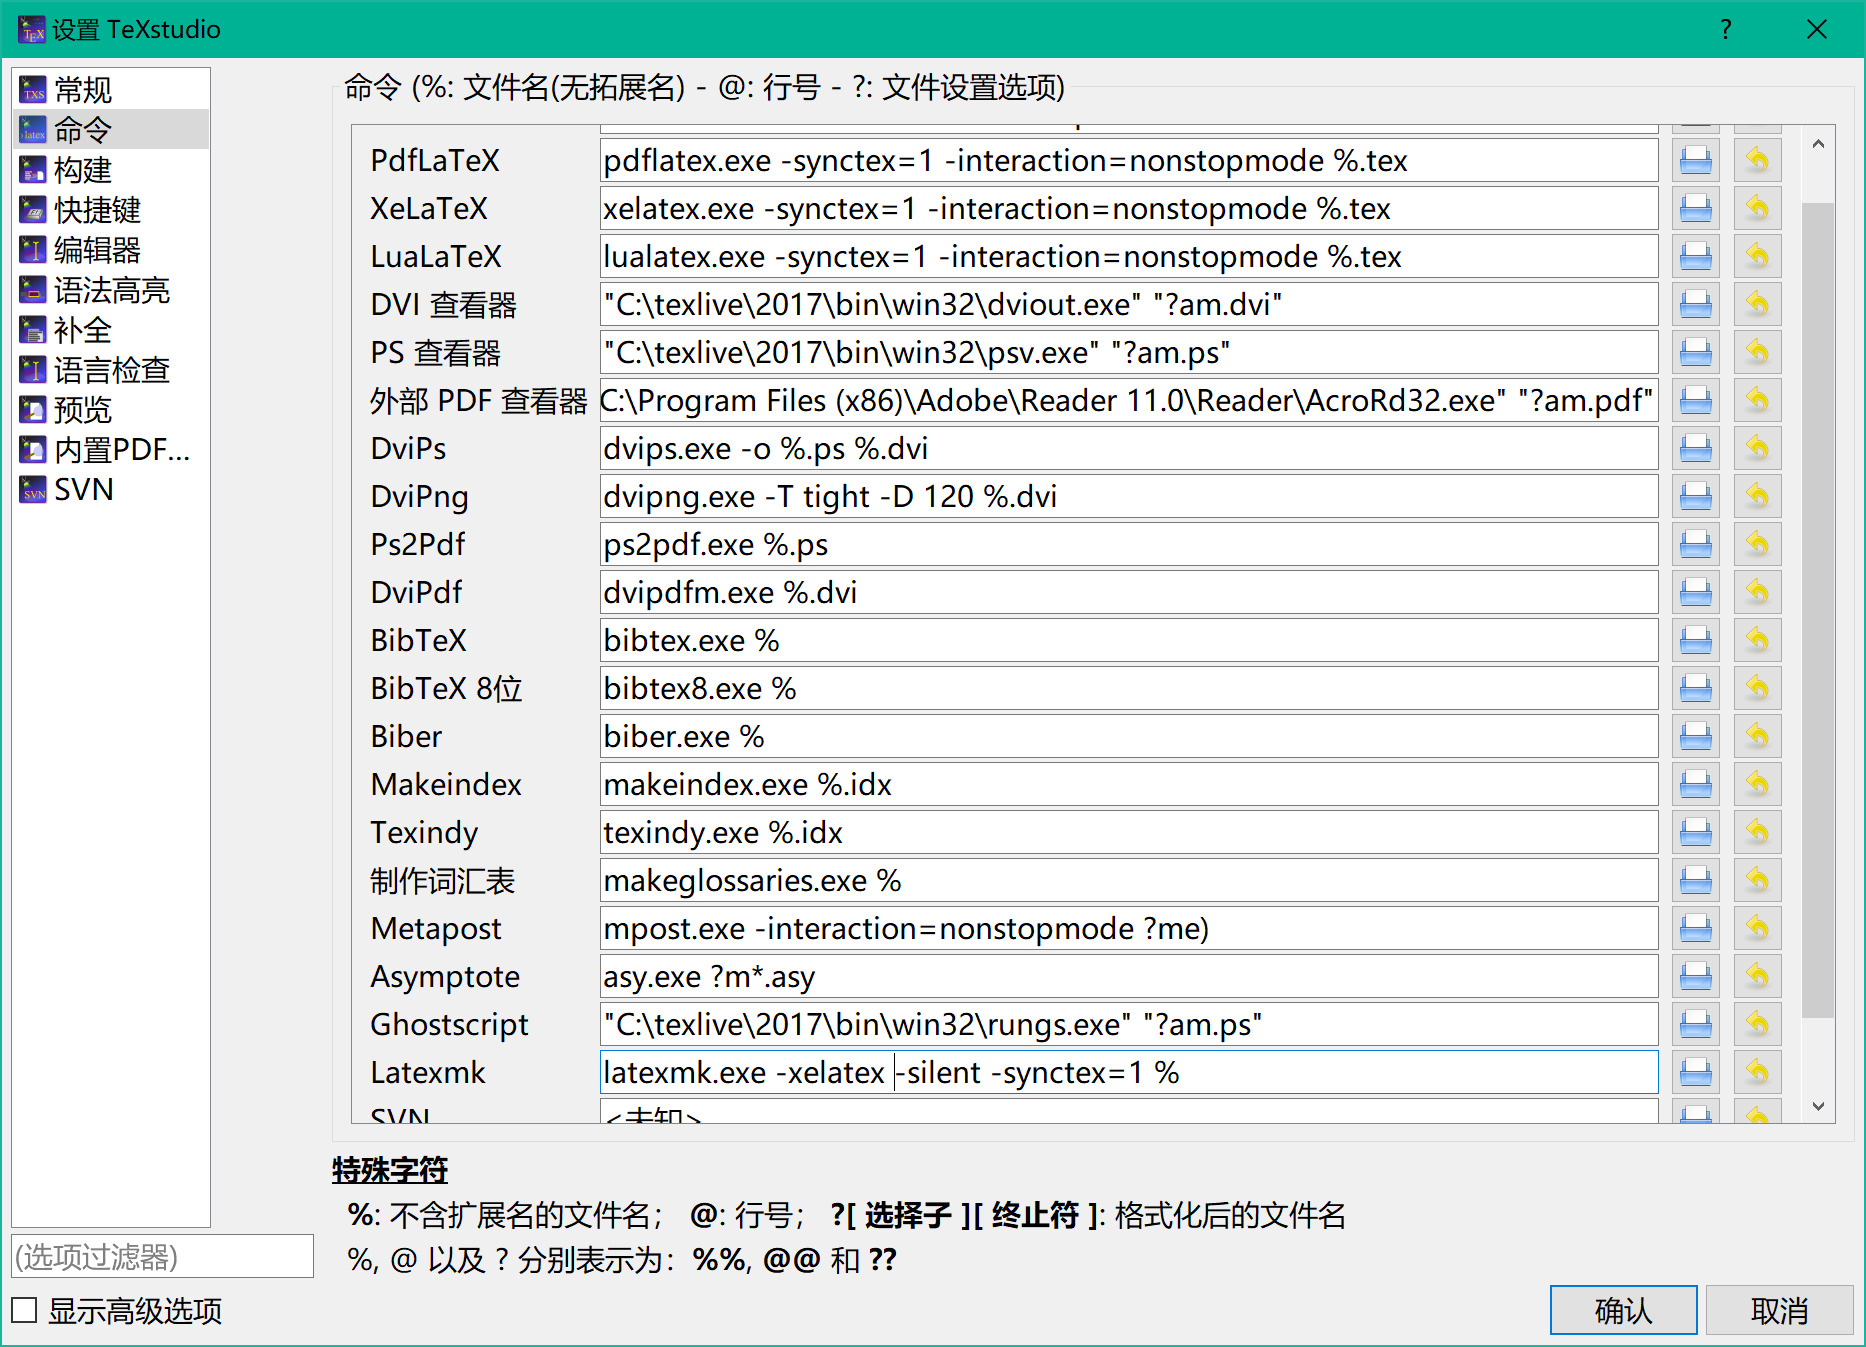
\includegraphics[width=0.45\textwidth]{texstudio-options-latexmk}}
    \annotatedFigureBox{0.005,0.88}{0.08,0.92}{red}
    \annotatedFigureBox{0.18,0.18}{0.8,0.23}{red}
    \annotatedFigureBox{0.405,0.184}{0.485,0.226}{blue}
  \end{annotatedFigure}
  \begin{annotatedFigure}
    {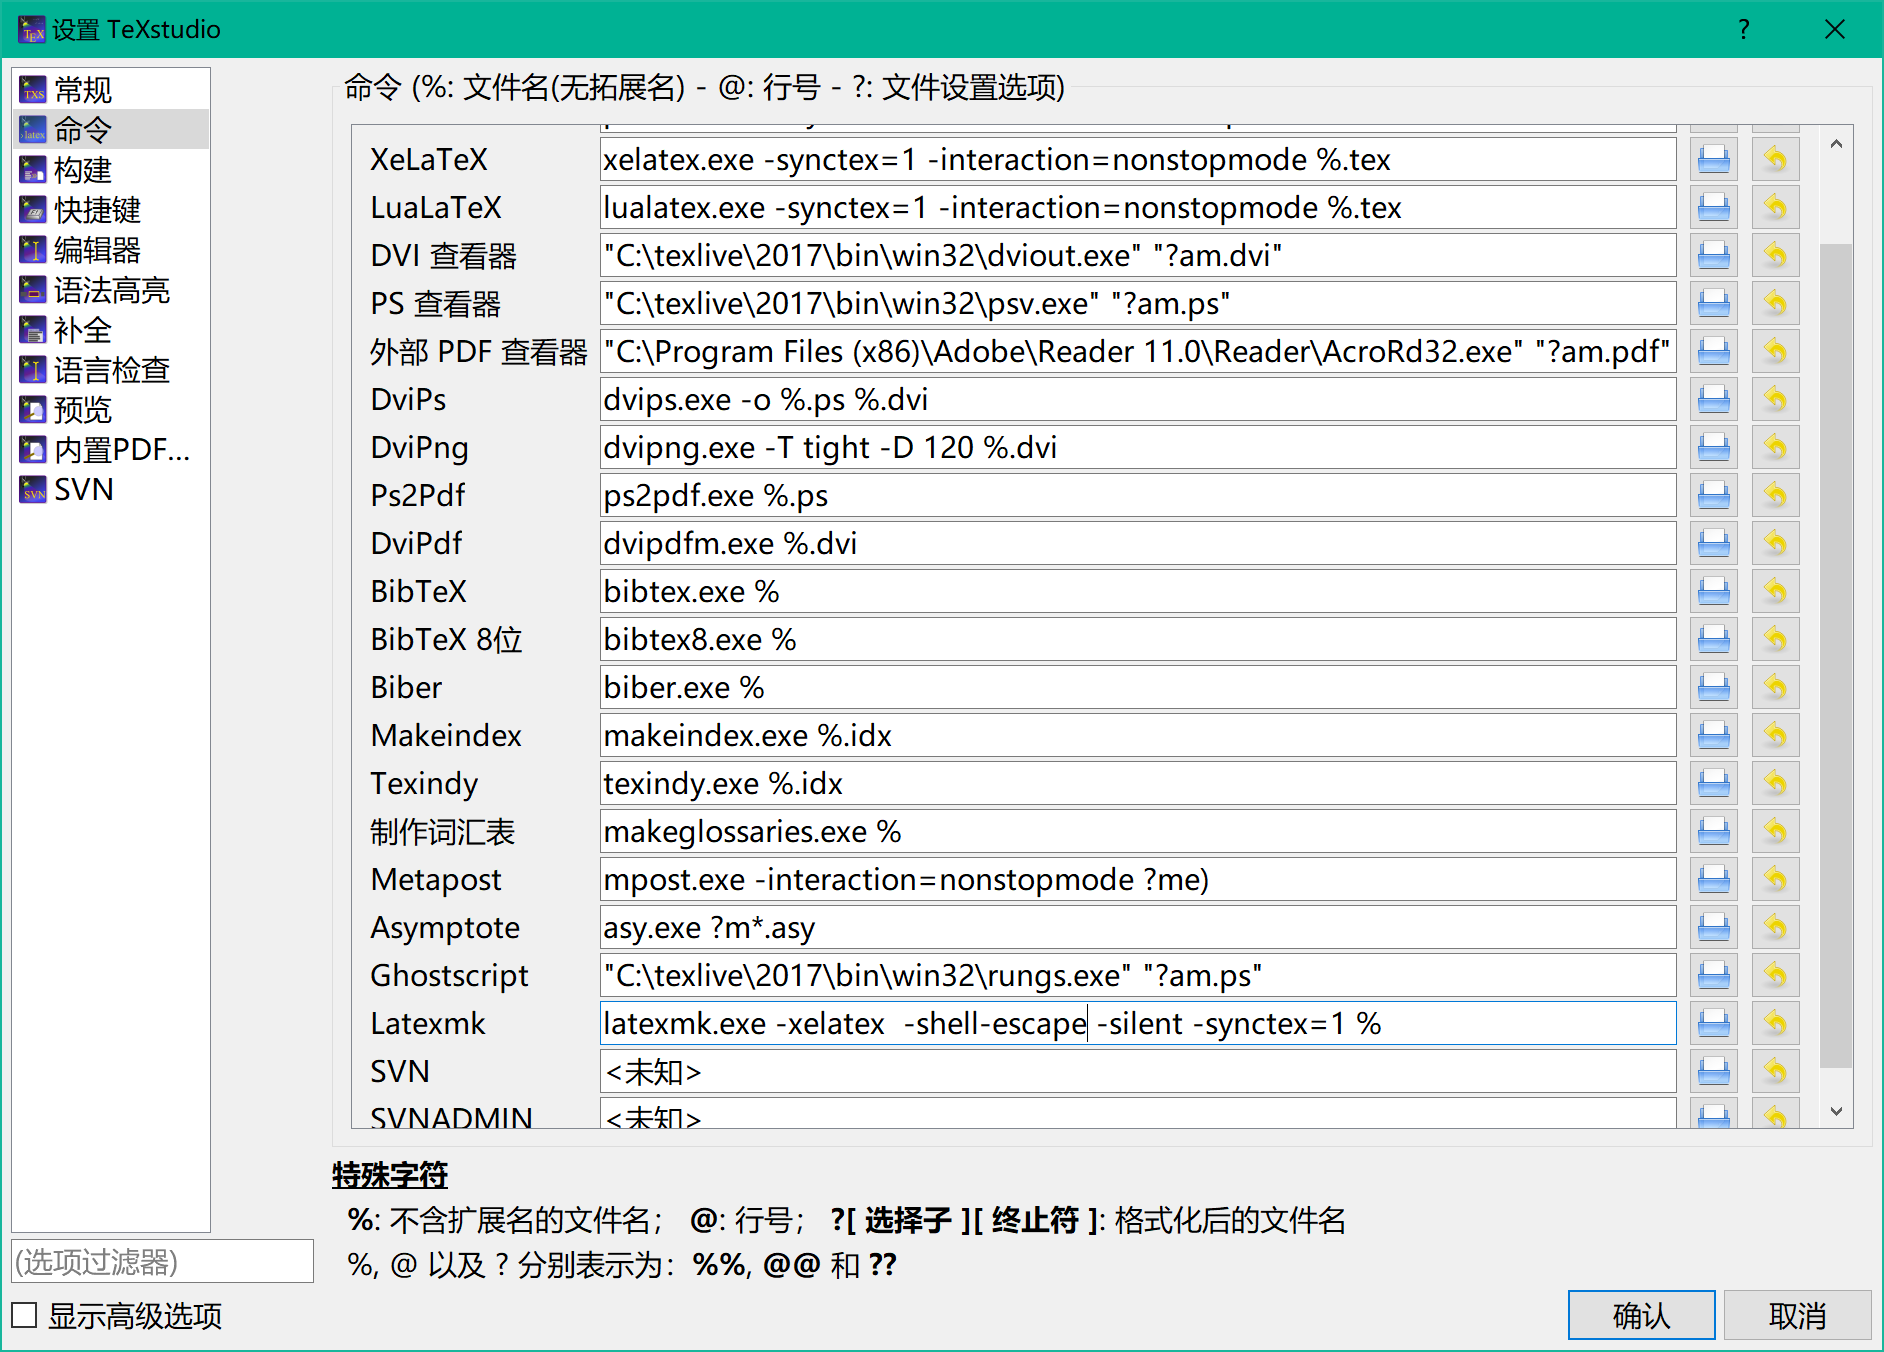
\includegraphics[width=0.45\textwidth]{texstudio-options-latexmk-withminted}}
    \annotatedFigureBox{0.005,0.88}{0.08,0.92}{red}
    \annotatedFigureBox{0.18,0.22}{0.8,0.27}{red}
    \annotatedFigureBox{0.47,0.224}{0.587,0.266}{blue}
  \end{annotatedFigure}  
  \stretchoff
\end{frame}

\begin{frame}{\nwafuprojrep 模板}{TeXstudio配置}
  \stretchon
  \begin{itemize}
  \item 用\pkg{latexmk} \alert{1次}编译(\alert{强烈推荐})
    \begin{enumerate}
    \item \pkg{latexmk} 编译\TeX 源码:\menu[,]{工具,构建并查看/F5}或\menu[,]{工具,编译/F6}
    \end{enumerate}
  \end{itemize}
  \centering
  \begin{annotatedFigure}
    {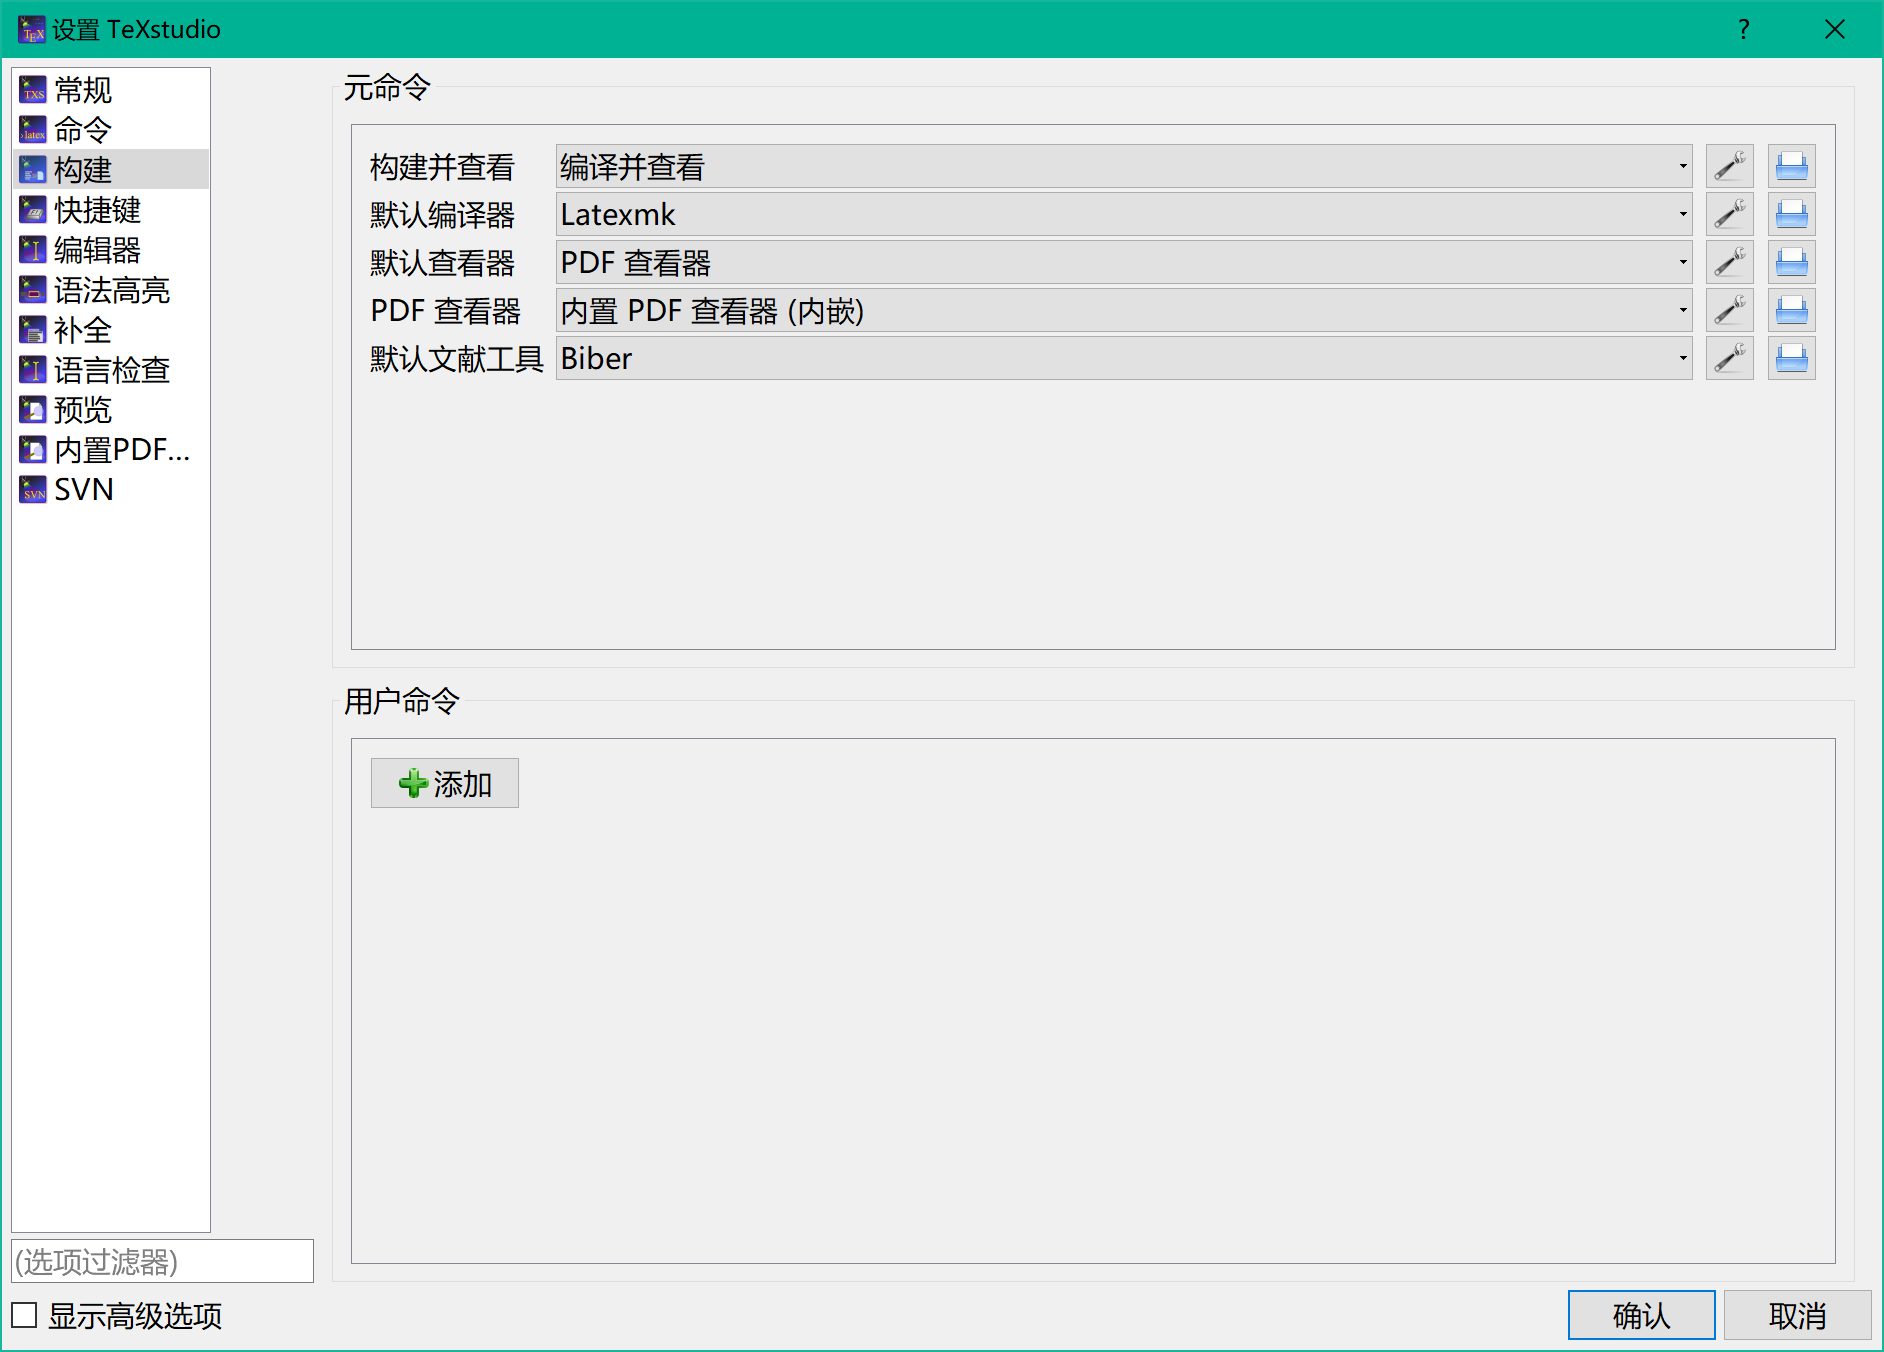
\includegraphics[width=0.65\textwidth]{texstudio-options-build-toolchains-latexmk-biber}}
    \annotatedFigureBox{0.005,0.855}{0.08,0.895}{red}
    \annotatedFigureBox{0.18,0.82}{0.4,0.86}{blue}
    \annotatedFigureBox{0.18,0.715}{0.4,0.755}{blue}
  \end{annotatedFigure}
  \stretchoff
\end{frame}

\begin{frame}{\nwafuprojrep 模板}{检测TeXstudio配置}
  \stretchon
  \begin{itemize}
  \item \menu[,]{帮助,检测\LaTeX 安装信息}
    
  \end{itemize}
  \centering
  \begin{annotatedFigure}
    {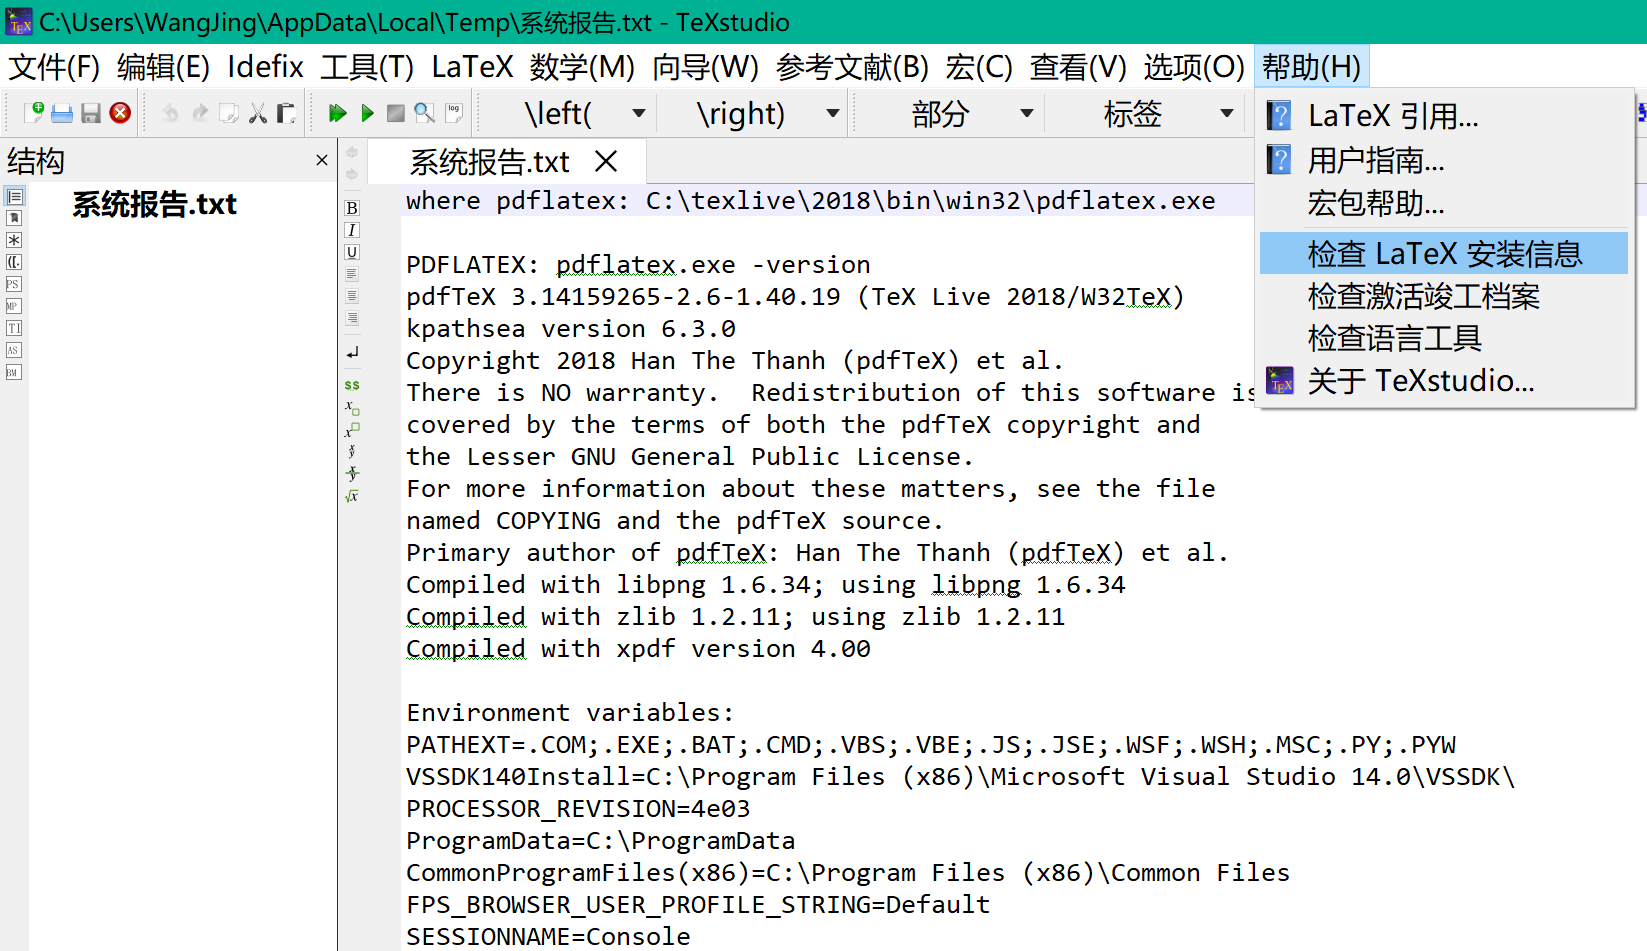
\includegraphics[width=0.75\textwidth]{texstudio-help-checklatex}}
    % \annotatedFigureBox{0.005,0.855}{0.08,0.895}{red}
    % \annotatedFigureBox{0.18,0.82}{0.4,0.86}{blue}
    % \annotatedFigureBox{0.18,0.715}{0.4,0.755}{blue}
  \end{annotatedFigure}
  \stretchoff
\end{frame}

\begin{frame}{\nwafuprojrep 模板}{宏包推荐\footnote[frame,3]{请务必先读文
      档:命令行执行\alert{\texttt{texdoc package}}}\footnote[frame,4]{本页面摘自曾祥东的\enquote{现代\LaTeX 入门讲座}
      讲义\link{https://github.com/stone-zeng/latex-talk}。}}
  \stretchon
  \footnotesize
  \setbeamertemplate{itemize/enumerate subbody begin}{\scriptsize}
  \setlength{\leftmarginii}{1.5em}
  \vspace{-18ex}
  \begin{multicols}{3}
    \begin{itemize}
    \item 必备

      \begin{itemize}
      \item \pkg{amsmath}(已加载)
      \item \pkg{graphicx}(已加载)
      \item \pkg{hyperref}
      \end{itemize}

    \item 样式

      \begin{itemize}
      \item \pkg{caption}(已加载)
      \item \pkg{enumitem}(已加载)
      \item \pkg{fancyhdr}(已加载)
      \item \pkg{footmisc}
      \item \pkg{geometry}(已加载)
      \item \pkg{ntheorem}
      \item \pkg{titlesec}
      \end{itemize}

    \item 数学

      \begin{itemize}
      \item \pkg{bm}
      \item \pkg{mathtools}
      \item \pkg{physics}
      \item \pkg{unicode-math}
      \end{itemize}

    \item 表格

      \begin{itemize}
      \item \pkg{array}
      \item \pkg{booktabs}
      \item \pkg{longtable}
      \item \pkg{tabularx}
      \end{itemize}

    \item 插图、绘图

      \begin{itemize}
      \item \pkg{floatrow}
      \item \pkg{pdfpages}
      \item \pkg{subfig}
      \item \pkg{pgf}/\pkg{tikz}
      \item \pkg{pgfplots}
      \end{itemize}

    \item 字体

      \begin{itemize}
      \item \pkg{newtx}
      \item \pkg{newpx}
      \item \pkg{pifont}
      \item \pkg{fontspec}
      \end{itemize}

    \item 各种功能

      \begin{itemize}
      \item \pkg{algorithm2e}
      \item \pkg{beamer}
      \item \pkg{biblatex}(已加载)
      \item \pkg{fancyhdr}(已加载)
      \item \pkg{listings}
      \item \pkg{mhchem}
      \item \pkg{microtype}
      \item \pkg{minted}
      \item \pkg{siunitx}
      \item \pkg{xcolor}
      \end{itemize}

    \item 多语言

      \begin{itemize}
      \item \pkg{babel}
      \item \pkg{polyglossia}
      \item \pkg{ctex}(已加载)
      \item \pkg{xeCJK}(已加载)
      \item \pkg{luatexja}
      \end{itemize}
    \end{itemize}
  \end{multicols}
  \vspace*{-0.5cm}
  \stretchoff
\end{frame}

\subsection[Git托管]{Git版本托管}
\begin{frame}{\nwafuprojrep 模板}{Git版本托管}
  %\stretchon
  \begin{itemize}
  \item 修订管理
    \begin{itemize}
    \item 注释管理
    \item 版本控制
      \begin{itemize}
      \item Git(回滚、diff)
      \end{itemize}
    \end{itemize}
  \end{itemize}
  \begin{center}
    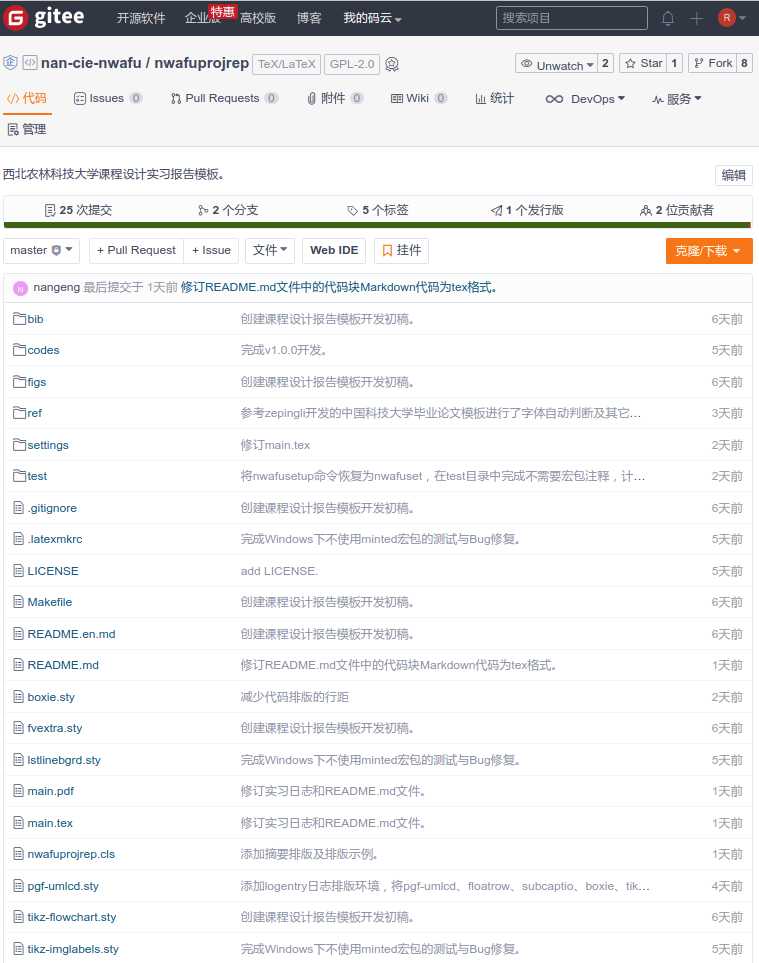
\includegraphics[height=0.65\textheight]{gitee}\quad
    \scalebox{0.8}{
      %  \begin{center}
    % \includegraphics[height=0.8\textheight]{coworks}
%    \scalebox{0.5}{
      \begin{forest}
        pic dir tree,
        pic root,
        for tree={% folder icons by default; override using file for file icons
          directory,
        },
        [jobname【projrep】%,
          [实习报告.docx, file]
          [实习报告改.docx, file]
          [实习报告改1.docx, file]
          [实习报告改2.docx, file]
          [实习报告最新版.docx, file]
          [实习报告最新版改.docx, file]
          [实习报告最终版.docx, file]
          [实习报告超级最终版.docx, file]
          [实习报告超级最终版改.docx, file]
          [实习报告绝对超级最终版.docx, file]
          [实习报告绝对超级最终版2.docx, file]
          [定稿???.docx, file]
        ]
      \end{forest}
%    }
%  \end{center}

    }
    %\includegraphics[height=0.6\textheight]{wordver02}\quad
    %\includegraphics[height=0.4\textheight]{wordver02}
  \end{center}
  %\stretchoff
\end{frame}

\begin{frame}[fragile]{\nwafuprojrep 模板}{Git版本托管
    \footnote[frame,1]{本页面摘自曾祥东的\enquote{现代\LaTeX 入门讲座}
      讲义\link{https://github.com/stone-zeng/latex-talk}。}}
  \stretchon
  \begin{itemize}
    \item 版本管理的必要性
      \begin{itemize}
        \item 远离「初稿,第二稿,第三稿……终稿,终稿(打死也不改了)」
        \item 有底气做大范围修改、重构
        \item 方便与他人协同合作
      \end{itemize}
    \item 基本用法
      \begin{itemize}
        \item 把大象放进冰箱:\shinline{git init}、\shinline{git add}、\shinline{git commit}
        \item 时空穿梭:\shinline{git reset}、\shinline{git revert}
        \item 平行宇宙:\shinline{git branch}、\shinline{git checkout}、\shinline{git rebase}
        %\item 推荐用\enquote{GitHub Desktop}、\enquote{VS Code}等软件进行可视化操作
        \item 参考链接:git-Book\link{https://git-scm.com/book/en/v2}
          或廖雪峰的git教程
          \link{https://www.liaoxuefeng.com/wiki/0013739516305929606dd18361248578c67b8067c8c017b000}
      \end{itemize}
    \item Gitee码云\href{https://gitee.com}或GitHub \href{https://github.com}{\faGithub}
      \begin{itemize}
        \item 远程 Git 仓库
        \item Clone \& fork
        \item Issues \& pull requests
        \item \alert{提醒}:GitHub绑定 \texttt{.edu} 邮箱可以免费无限量使用私有仓库
      \end{itemize}
  \end{itemize}
  \stretchoff
\end{frame}

%%%%%%%%%%%%%%%%%%%%%%%%%%%%%% 参考文献 %%%%%%%%%%%%%%%%%%%%%%%%%%%%%%%%%%%
\section[参考文献]{参考文献}
\begin{frame}[fragile]{参考文献}{学无止境\footnote[frame,1]{感谢现代
      \LaTeX 入门讲座作者曾祥东的汇总整理,本文中的\texinline[fontsize
      = \zihao{7}]{\link}等
      命令也来自该文档,在此一并对作者致以衷心的感谢!\link{https://github.com/stone-zeng/latex-talk}}}
\begin{multicols}{2}
\tiny
\newcommand\BOOK[1]{\textbf{#1}}
\newcommand\TAG[1]{\CASE{[#1]}}
\begin{thebibliography}{99}
  \bibitem{}
    \textsc{Knuth D E}.
    \newblock \BOOK{The \TeX book: Computers \& Typesetting, volume C} \TAG{M}. 1984.
    \newblock Boston: Addison--Wesley Publishing Company
  \bibitem{}
    刘海洋.
    \newblock \BOOK{\LaTeX{} 入门} \TAG{M}. 2013.
    \newblock 北京:电子工业出版社
  \bibitem{}
    \jatext{高冈昌生}.\\
    翻译:刘庆,监修:陈嵘.
    \newblock \BOOK{西文排版:排版的基础和规范} \TAG{M}. 2016.
    \newblock 北京:中信出版集团
  \bibitem{}
    \jatext{小林章}.\\
    翻译:刘庆,监修:陈嵘.
    \newblock \BOOK{西文字体:字体的背景知识和使用方法} \TAG{M}. 2014.
    \newblock 北京:中信出版集团
  \bibitem{}
    \textsc{Oetiker T}, \textsc{Partl H}, \textsc{Hyna I} and \textsc{Schlegl E}.\\
    翻译:\CTeX{} 开发小组.
    \newblock \BOOK{一份(不太)简短的 \LaTeXe{} 介绍:或 106 分钟了解 \LaTeXe{}} \TAG{EB/OL}. 2018.
    \newblock \url{https://ctan.org/pkg/lshort-zh-cn}
  \bibitem{}
    汪彧之,陈晟祺.
    \newblock \BOOK{如何使用 \LaTeX{} 排版论文} \TAG{EB/OL}. 2018.
    \newblock PDF:
      \href{https://github.com/tuna/thulib-latex-talk/raw/master/latex-talk.pdf}{\faDownload}
  \bibitem{}
    刘海洋.
    \newblock \BOOK{\LaTeX{} 入门} \TAG{EB/OL}. 2013.
    \newblock PDF:
      \href{https://bbs.pku.edu.cn/attach/e7/f2/e7f2bb698b9c3672/tex_intro_talk.pdf}{\faDownload}
  \bibitem{}
    林莲枝.
    \newblock \BOOK{漫谈 \LaTeX{} 排版常见概念误区:别把 \LaTeX{} 当 Word 用!}\TAG{EB/OL}. 2018.
    \newblock PDF:
      \href{http://static.latexstudio.net/wp-content/uploads/2018/03/LianTze-presentation-0320-forReading.pdf}{\faDownload}
  \bibitem{}
    Wikibooks.
    \newblock \BOOK{\LaTeX{}---Wikibooks, The Free Textbook Project} \TAG{EB/OL}.
    \newblock \url{https://en.wikibooks.org/wiki/LaTeX}
  \bibitem{}
    Overleaf.
    \newblock \BOOK{Overleaf Documentation} \TAG{EB/OL}.
    \newblock \url{https://www.overleaf.com/learn}
  \bibitem{}
    刘庆.
    \newblock \BOOK{孔雀计划:中文字体排印的思路} \TAG{EB/OL}.
    \newblock \url{https://thetype.com/kongque}
\end{thebibliography}
\end{multicols}
%\nonumberfootnote{fsdafasdfddddd}
\end{frame}

% 封底
%%%%%%%%%%%%%%%%

{
  \nwsuafwavesbg
  \begin{frame}[plain,noframenumbering]
    \finalpage{
      娟秀轻爽拉泰赫\\
      所写所想即所得\\
      排版何须穷思量\\
      窈窕俊俏尽婀娜\\
      \vspace{4ex}
      谢谢你使用该{\LaTeX} 简单教程!\\
      欢迎多提宝贵意见和建议}
  \end{frame}
}
%%%%%%%%%%%%%%%%
\end{document}

%%% Local Variables:
%%% mode: latex
%%% TeX-master: t
%%% End:
